%%
%% This is file `sample-sigconf.tex',
%% generated with the docstrip utility.
%%
%% The original source files were:
%%
%% samples.dtx  (with options: `all,proceedings,bibtex,sigconf')
%% 
%% IMPORTANT NOTICE:\input{sample-sigconf-kdd-2026}
%% 
%% 
%% For the copyright see the source file.
%% 
%% Any modified versions of this file must be renamed
%% with new filenames distinct from sample-sigconf.tex.
%% 
%% For distribution of the original source see the terms
%% for copying and modification in the file samples.dtx.
%% 
%% This generated file may be distributed as long as the
%% original source files, as listed above, are part of the
%% same distribution. (The sources need not necessarily be
%% in the same archive or directory.)
%%
%%
%% Commands for TeXCount
%TC:macro \cite [option:text,text]
%TC:macro \citep [option:text,text]
%TC:macro \citet [option:text,text]
%TC:envir table 0 1
%TC:envir table* 0 1
%TC:envir tabular [ignore] word
%TC:envir displaymath 0 word
%TC:envir math 0 word
%TC:envir comment 0 0
%%
%% The first command in your LaTeX source must be the \documentclass
%% command.
%%
%% For submission and review of your manuscript please change the
%% command to \documentclass[manuscript, screen, review]{acmart}.
%%
%% When submitting camera ready or to TAPS, please change the command
%% to \documentclass[sigconf]{acmart} or whichever template is required
%% for your publication.
%%
%%
%\documentclass[sigconf]{acmart}
\documentclass[sigconf,review]{acmart}
\usepackage{comment}
\usepackage[export]{adjustbox}
\usepackage{stfloats}
\usepackage{afterpage}
\usepackage{tikz}
\usepackage{fontawesome5}
\usepackage{booktabs}
\usepackage{rotating}
\usepackage{makecell}
\usepackage[table]{xcolor}
\definecolor{highlight}{gray}{0.95}

%%
%% \BibTeX command to typeset BibTeX logo in the docs
\AtBeginDocument{%
  \providecommand\BibTeX{{%
    Bib\TeX}}}

%% Rights management information.  This information is sent to you
%% when you complete the rights form.  These commands have SAMPLE
%% values in them; it is your responsibility as an author to replace
%% the commands and values with those provided to you when you
%% complete the rights form.
\setcopyright{acmlicensed}
\copyrightyear{2026}
\acmYear{2026}
\acmDOI{XXXXXXX.XXXXXXX}
%% These commands are for a PROCEEDINGS abstract or paper.
\acmConference[KDD '26] {The 32nd ACM SIGKDD Conference on Knowledge Discovery and Data Mining} {August 9--13, 2026} {Jeju, South Korea}
%%
%%  Uncomment \acmBooktitle if the title of the proceedings is different
%%  from ``Proceedings of ...''!
%%
%%\acmBooktitle{Woodstock '18: ACM Symposium on Neural Gaze Detection,
%%  June 03--05, 2018, Woodstock, NY}
\acmISBN{978-1-4503-XXXX-X/2018/06}


%%
%% Submission ID.
%% Use this when submitting an article to a sponsored event. You'll
%% receive a unique submission ID from the organizers
%% of the event, and this ID should be used as the parameter to this command.
%%\acmSubmissionID{123-A56-BU3}

%%
%% For managing citations, it is recommended to use bibliography
%% files in BibTeX format.
%%
%% You can then either use BibTeX with the ACM-Reference-Format style,
%% or BibLaTeX with the acmnumeric or acmauthoryear sytles, that include
%% support for advanced citation of software artefact from the
%% biblatex-software package, also separately available on CTAN.
%%
%% Look at the sample-*-biblatex.tex files for templates showcasing
%% the biblatex styles.
%%

%%
%% The majority of ACM publications use numbered citations and
%% references.  The command \citestyle{authoryear} switches to the
%% "author year" style.
%%
%% If you are preparing content for an event
%% sponsored by ACM SIGGRAPH, you must use the "author year" style of
%% citations and references.
%% Uncommenting
%% the next command will enable that style.
% KDD is all number system
% \citestyle{acmauthoryear}

%%
%% end of the preamble, start of the body of the document source.
\begin{document}
\title{PHMForge: A Scenario-Driven Agentic Benchmark for Industrial Asset Lifecycle Maintenance}

\author{Ayan Das}
\email{adas446@gatech.edu}
\affiliation{%
  \institution{Georgia Institute of Technology}
  \country{USA}
}

\author{Dhaval Patel}
\email{pateldha@us.ibm.com}
\affiliation{%
  \institution{IBM}
  \country{USA}
}
\renewcommand{\shortauthors}{Das et al.}
% \renewcommand{\shortauthors}{Das et al.}

\begin{abstract}
Large language model (LLM) agents are increasingly deployed for complex tool-orchestration tasks, yet existing benchmarks fail to capture the rigorous demands of industrial domains where incorrect decisions carry significant safety and financial consequences. To address this critical gap, we introduce PHMForge, the first comprehensive benchmark specifically designed to evaluate LLM agents on Prognostics and Health Management (PHM) tasks through realistic interactions with domain-specific MCP servers. Our benchmark encompasses 75 expert-curated scenarios spanning 7 industrial asset classes (turbofan engines, bearings, electric motors, gearboxes, aero-engines) across 5 core task categories: Remaining Useful Life (RUL) Prediction, Fault Classification, Engine Health Analysis, Cost-Benefit Analysis, and Safety/Policy Evaluation. To enable rigorous evaluation, we construct 22 specialized tools across two MCP servers and implement execution-based evaluators with task-commensurate metrics: MAE/RMSE for regression, F1-score for classification, and categorical matching for health assessments. Through extensive evaluation of leading frameworks (ReAct, Cursor Agent, Claude Code) paired with frontier LLMs (Claude Sonnet 4.0, GPT-4o, Granite-3.0-8B), we find that even top-performing configurations achieve only 68\% task completion, with systematic failures in tool orchestration (23\% incorrect sequencing), multi-asset reasoning (14.9 percentage point degradation), and cross-equipment generalization (42.7\% on held-out datasets). Our benchmark introduces an unknown-tools challenge, as agents must retrieve appropriate functions from vague industrial queries without explicit tool names, mirroring real deployment scenarios. Following a living benchmark philosophy with progressive SME-driven curation (396 person-hours across domain experts), PHMForge is designed for continuous expansion as new industrial assets and failure modes emerge. We open-source our complete benchmark, including scenario specifications, ground truth templates, tool implementations, and evaluation scripts, to catalyze research in agentic industrial AI.
\end{abstract}

\begin{teaserfigure}
   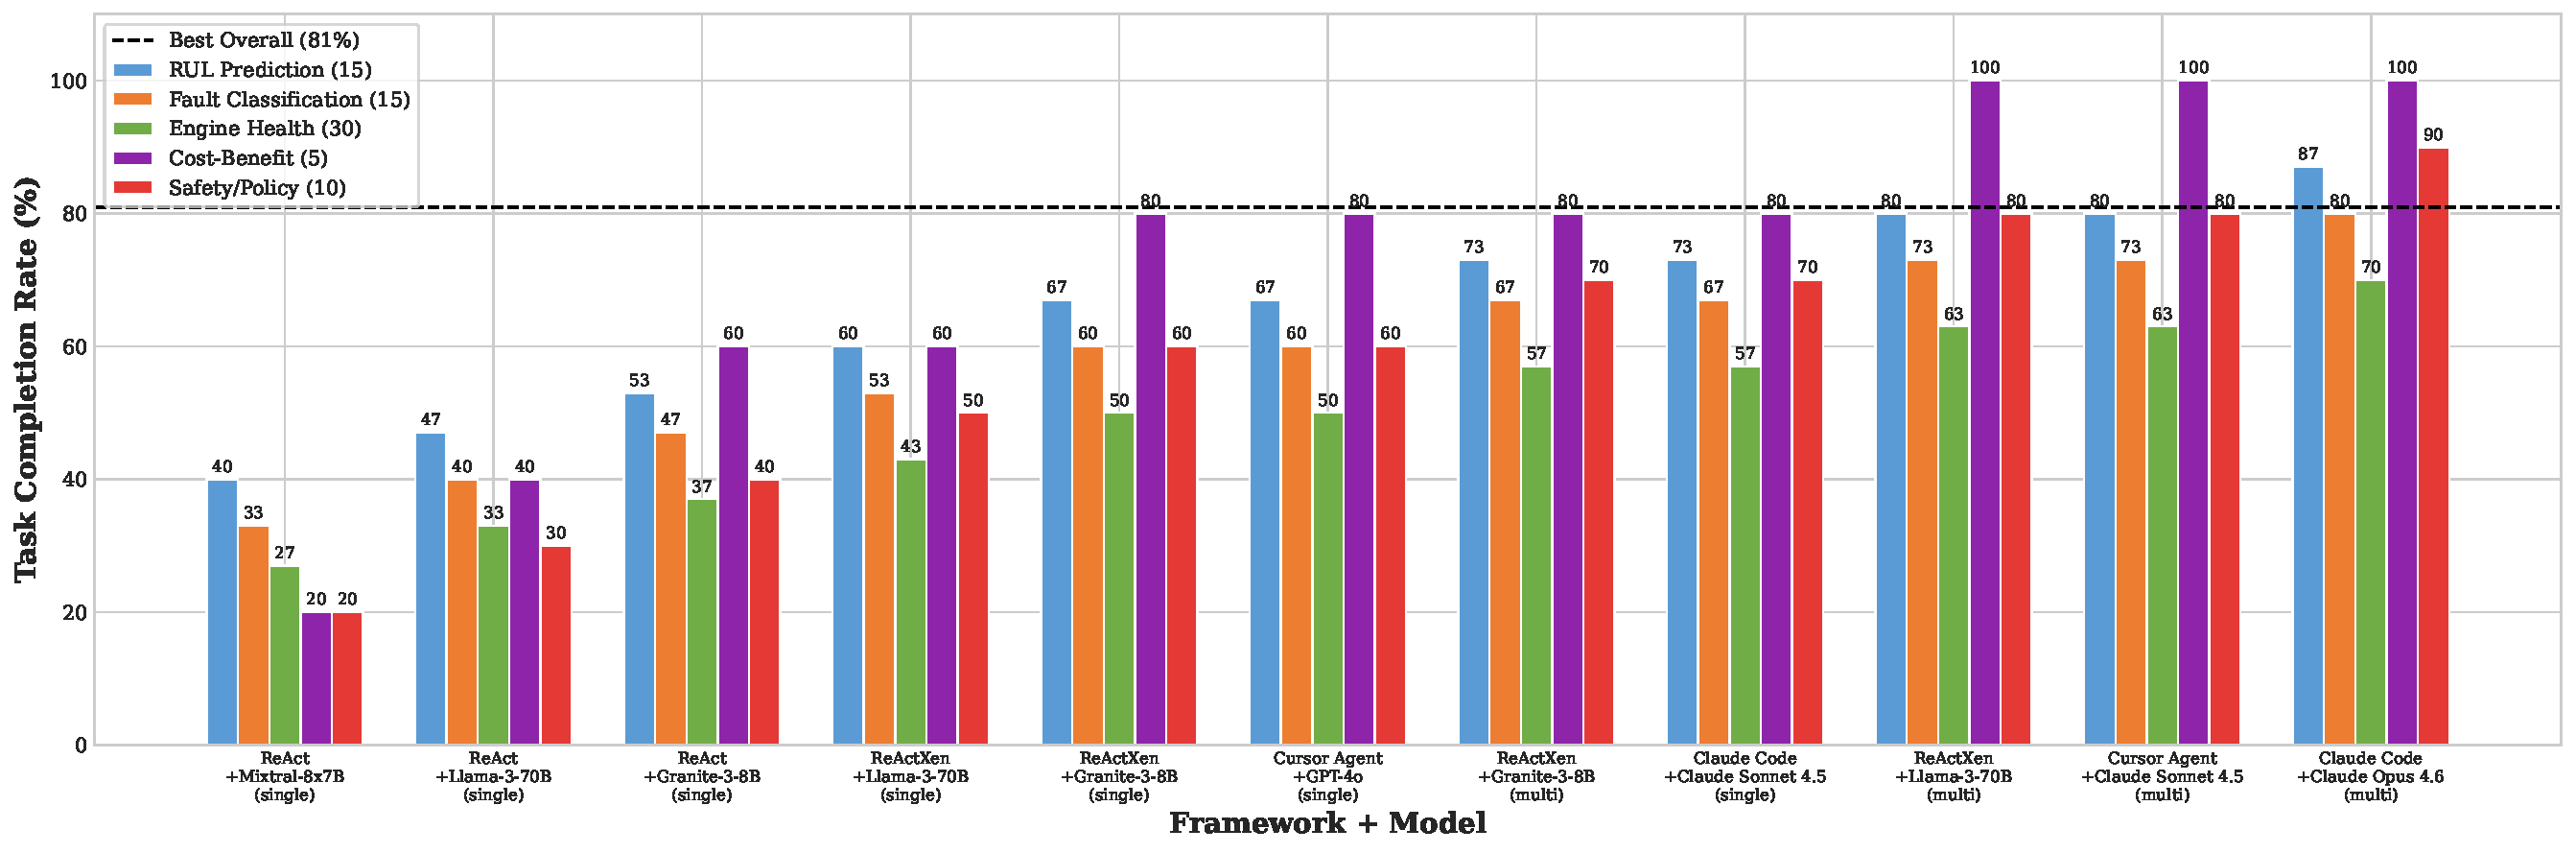
\includegraphics[width=\textwidth]{agentic_performance_chart}
   \caption{PHMForge benchmark results across framework-model combinations. Even top configurations (Claude Code + Sonnet 4.0) achieve only 68\% task completion, with Engine Health Analysis proving most challenging (23.3--60.0\% range). Task categories: RUL Prediction (15 scenarios), Fault Classification (15 scenarios), Health Analysis (30 scenarios).}
   \Description{Bar chart comparing task completion rates across seven framework-model combinations on three PHM task categories, showing frontier models achieving 60-80\% on individual tasks but struggling with overall benchmark completion.}
   \label{fig:teaser}
\end{teaserfigure}

%%
%% The code below is generated by the tool at http://dl.acm.org/ccs.cfm.
%% Please copy and paste the code instead of the example below.
%%
\begin{CCSXML}
<ccs2012>
   <concept>
       <concept_id>10002951.10003227.10003228</concept_id>
       <concept_desc>Information systems~Enterprise information systems</concept_desc>
       <concept_significance>500</concept_significance>
       </concept>
   <concept>
       <concept_id>10010147.10010257</concept_id>
       <concept_desc>Computing methodologies~Machine learning</concept_desc>
       <concept_significance>500</concept_significance>
       </concept>
 </ccs2012>
\end{CCSXML}

\ccsdesc[500]{Information systems~Enterprise information systems}
\ccsdesc[500]{Computing methodologies~Machine learning}

%%
%% Keywords. The author(s) should pick words that accurately describe
%% the work being presented. Separate the keywords with commas.
% place set of keywords here
\keywords{Stakeholder-Aligned Taxonomy, Multi-Modal Orchestration, Cross-Platform Empirical Calibration, Deterministic Ground-Truth Verification, Multi-Hop Query Disambiguation}

\maketitle


\section{Introduction}

Industrial Artificial Intelligence (Industrial AI) represents the systematic integration of machine learning and data mining into physical ecosystems to enhance the resilience, efficiency, and safety of critical assets \cite{9378369}. Unlike general-purpose AI, Industrial AI operates in high-stakes environments where the "cost of failure" is not merely a digital error, but potentially catastrophic equipment damage, environmental impact, or risks to human life. Central to this field is \textbf{Prognostics and Health Management (PHM)} \cite{PHMbook}, which focuses on the end-to-end lifecycle of physical assets, ranging from turbofan engines to industrial gearboxes.

% need to give an example of kaggle-style competition here.
Historically, the path to a functional PHM system has been an arduous, manual process for data scientists. In the traditional paradigm, often mirrored in \textbf{Kaggle-style} competitions \cite{ibm_enterprise_ops_2025}, experts manually curate datasets, perform exhaustive feature engineering for specific sensor modalities, and tune black-box models for isolated tasks like Remaining Useful Life (RUL) prediction \cite{hamilton2026neurosymbolicaipredictivemaintenance}. A key driver for this research has been the aggregation of diverse data, such as the collection of over 100 industrial datasets \cite{vanderVenIndustrialDatasets}. While these ad-hoc approaches yield results in controlled settings, they create a ``deployment bottleneck'': they require intensive human-in-the-loop orchestration for every new asset class and fail to scale to the heterogeneous, multi-modal, and high-dimensional sensor streams characteristic of \textbf{Industry 5.0} deployments \cite{wang2025itformer, yang2025phmbenchdomainspecificbenchmarkingframework}.

The recent emergence of \textbf{Large Language Model (LLM) agents} for autonomous task orchestration offers a transformative path toward automating this complex lifecycle. These systems leverage agentic frameworks such as \textbf{ReAct}~\cite{yao2023reactsynergizingreasoningacting}, which enable models to interleave reasoning and acting in response to real-time feedback. Concurrently, standardized protocols like the \textbf{Model Context Protocol (MCP)}~\cite{mcp_intro_2024} provide consistent tool invocation schemas, enabling multi-hop workflows that chain specialized functions across disparate industrial domains~\cite{wang2025mcpbenchbenchmarkingtoolusingllm}. 

However, adapting these promising agent architectures to industrial settings exposes fundamental gaps in existing evaluation infrastructure. While existing benchmarks such as \textbf{StableToolBench}~\cite{guo2025stabletoolbenchstablelargescalebenchmarking}, \textbf{MLE-Bench}~\cite{chan2025mlebenchevaluatingmachinelearning}, and \textbf{MCP-Universe}~\cite{luo2025mcpuniversebenchmarkinglargelanguage} evaluate agents on isolated API calls or general data science tasks, they fail to address the rigorous, domain-specific demands of PHM. Diagnosing bearing faults across heterogeneous sensor modalities or orchestrating maintenance decisions requires integrating technical diagnostics with strict operational standards (e.g., ISO 55000). To bridge this gap, \textbf{AssetOpsBench}~\cite{patel2025assetopsbenchbenchmarkingaiagents} has recently emerged as a domain-authentic benchmark that moves beyond synthetic tasks to evaluate agents on long-term asset lifecycles and complex, multi-modal reasoning. Yet, the absence of standardized, unified frameworks to evaluate the \emph{interplay} between emerging protocols (i.e., MCPs) and safety-critical constraints leaves practitioners unable to assess whether frontier LLMs can truly navigate the high-stakes dependencies of the physical world.
To address this critical gap, we introduce \textbf{PHMForge}, the first comprehensive benchmark specifically designed to evaluate LLM agents on industrial asset lifecycle maintenance through realistic interactions with domain-specific MCP servers. Our contributions are summarized as follows:
\begin{itemize}
    \item \textbf{Comprehensive Industrial Scope:} PHMForge encompasses 75 expert-curated scenarios spanning 7 asset classes (including turbofan engines, electric motors, and gearboxes) across 5 core PHM task categories.
    \item \textbf{Specialized Tooling Infrastructure:} We construct 22 specialized tools across two MCP servers, namely the \textit{Prognostics Server} and the \textit{Intelligent Maintenance Server}, to enable evaluation on tasks where no standardized tooling previously existed.
    \item \textbf{The Unknown-Tools Challenge:} We introduce a novel evaluation mode where agents must retrieve appropriate functions from vague industrial queries (e.g., \textit{``Which engines in our fleet are nearing critical limits?''}), requiring multi-hop reasoning and domain-specific intent extraction.
    \item \textbf{Systematic Evaluation:} Through extensive testing of leading frameworks (ReAct, Cursor Agent \cite{cursor_docs}) and frontier LLMs (Claude Sonnet 4.0 \cite{claude_sonnet_docs}, GPT-4o \cite{gpt_4o}), we identify systematic failures in tool sequencing (23\%) and cross-equipment generalization (42.7\%), establishing a baseline for future research.
\end{itemize}

Following a living benchmark philosophy inspired by \textbf{TabArena} \cite{erickson2025tabarenalivingbenchmarkmachine}, \textsc{PHMForge} is designed for continuous expansion through progressive SME-driven curation. We open-source our complete benchmark, including scenario specifications, tool implementations, and evaluation scripts, to catalyze the development of reliable, agentic Industrial AI.

\begin{center}
\textbf{\textcolor{purple}{\faFile}\ \href{https://github.com/DeveloperMindset123/Intent-Based-Industrial-Automation/blob/scenarios_and_datasets/ReActXen/src/reactxen/demo/intent_implementation_demo/scenario/my_scenarios.json}{Dataset}} \quad
\textbf{\textcolor{teal}{\faLaptopCode}\ \href{https://github.com/DeveloperMindset123/Intent-Based-Industrial-Automation}{GitHub}} \quad
\textbf{\textcolor{teal}{\faRocket}\ \href{https://phmforge.streamlit.app/}{Live Demo}}
\end{center}


% --- Figure Placeholder ---
\begin{figure*}
    \centering
    \includegraphics[width=0.85\textwidth]{PHMArchitectureDiagram.png}
\caption{\textbf{PHMForge Architecture.} Industrial stakeholder queries are processed by agentic frameworks and LLM backbones, which orchestrate tools across two domain-specific MCP servers: the \textbf{Prognostics Server} (15 tools for RUL, fault classification, and health analysis) and the \textbf{Intelligent Maintenance Server} (7 tools for cost-benefit and safety evaluation).}
    \label{fig:architecture}
\end{figure*}
% \section{Scenarios Categorization : Mapping to PHM Core Tasks}

\section{Related Work and Research Positioning}

The evaluation of intelligent systems in industrial contexts is evolving from static model assessment to agentic orchestration. We categorize prior work into three pillars and identify the fundamental gaps addressed by \textbf{PHMForge}.

\subsection{PHM Benchmarks and Time-Series QA}
Traditional PHM research focuses on standardized model performance. \textbf{PDMBench}~\cite{anonymous2026pdmbench} provides an extensive platform for evaluating 22 models across 14 datasets for fault classification and RUL prediction. Recently, efforts have moved toward multi-modal interfaces; \textbf{ITFormer}~\cite{wang2025itformer} introduced \textit{EngineMT-QA}, a large-scale dataset for aero-engine question answering. Similarly, \textbf{PHM-Bench}~\cite{yang2025phmbenchdomainspecificbenchmarkingframework} proposed a three-dimensional framework to evaluate model lifecycle capabilities.
\textbf{Gap:} These benchmarks focus on \textit{passive evaluation} (QA or prediction accuracy) rather than \textit{active orchestration}. ITFormer relies on LLM-generated queries that lack in-depth SME (Subject Matter Expert) validation, while most datasets focus on isolated assets, limiting cross-equipment generalization.

\subsection{Language Agent Frameworks}
The \textbf{ReAct} paradigm~\cite{yao2023reactsynergizingreasoningacting} (interleaving reasoning and acting) has become the de facto standard for agentic workflows, achieving success in software engineering~\cite{yang2024sweagentagentcomputerinterfacesenable} and cloud operations~\cite{shetty2024buildingaiagentsautonomous}. 
\textbf{Gap:} Standard ReAct implementations assume static toolsets. \textbf{PHMForge} addresses this by introducing a ``dynamic tool discovery'' challenge where agents must autonomously retrieve and ground specialized PHM tools from an unfamiliar, high-stakes environment.

\subsection{Agentic and Tool-Use Benchmarks}
As Large Language Models (LLMs) evolve into autonomous agents, evaluation frameworks have shifted toward assessing their capacity for tool-mediated problem-solving. \textbf{MLE-Bench}~\cite{chan2025mlebenchevaluatingmachinelearning} benchmarks agents on machine learning engineering, while \textbf{MCP-Bench}~\cite{wang2025mcpbenchbenchmarkingtoolusingllm} and \textbf{MCP-Universe}~\cite{luo2025mcpuniversebenchmarkinglargelanguage} utilize the Model Context Protocol (MCP) to evaluate multi-step reasoning in generic domains such as finance and travel. Within the industrial sector, \textbf{ReActXen}~\cite{patel2025react} explores agentic interactions with SCADA systems. The most relevant antecedent is \textbf{AssetOpsBench}~\cite{patel2025assetopsbenchbenchmarkingaiagents}, which focuses on multi-agent orchestration; however, its scope is largely restricted to anomaly detection and historical work order analysis. Current agentic benchmarks remain predominantly ``digital-native.'' They fail to account for the high-dimensional, temporally-dependent sensor streams inherent to physical assets or the stringent regulatory constraints (e.g., OSHA, FAA) governing industrial maintenance. Furthermore, existing frameworks seldom address the cross-asset comparative analysis required for complex PHM workflows, specifically the orchestration across multiple instances of an asset class nor do they leverage standardized, emerging architectures like MCP to handle industrial telemetry.

\begin{table}[t!]
\centering
\small
\caption{Comparison of PHMForge with Existing Benchmarks}
\label{tab:comparison}
\setlength{\tabcolsep}{8pt} % Adjust spacing between columns
\begin{tabular}{l cccccc}
\toprule
& \multicolumn{6}{c}{\textbf{Benchmark Capabilities}} \\
\cmidrule{2-7}
\textbf{Benchmark} & 
\rotatebox{90}{\textbf{Expert-Vetted}} & 
\rotatebox{90}{\textbf{Multi-Asset}} & 
\rotatebox{90}{\textbf{Agentic}} & 
\rotatebox{90}{\textbf{PHM-Domain}} & 
\rotatebox{90}{\textbf{Dynamic Tools}} & 
\rotatebox{90}{\textbf{Det. Eval}} \\ 
\midrule
ITFormer~\cite{wang2025itformer} & $\times$ & $\times$ & $\times$ & $\checkmark$ & $\times$ & $\checkmark$ \\
MLE-Bench~\cite{chan2025mlebenchevaluatingmachinelearning} & $\times$ & N/A & $\checkmark$ & $\times$ & $\times$ & $\checkmark$ \\
PHM-Bench~\cite{yang2025phmbenchdomainspecificbenchmarkingframework} & ? & $\times$ & $\times$ & $\checkmark$ & $\times$ & ? \\
PDMBench~\cite{anonymous2026pdmbench} & ? & $\checkmark$ & $\times$ & $\checkmark$ & $\times$ & $\checkmark$ \\
MCP-Bench~\cite{wang2025mcpbenchbenchmarkingtoolusingllm} & $\times$ & N/A & $\checkmark$ & $\times$ & $\times$ & ? \\
ReActXen~\cite{patel2025react} & ? & N/A & $\checkmark$ & $\checkmark$ & $\times$ & ? \\
AssetOpsBench~\cite{patel2025assetopsbenchbenchmarkingaiagents} & $\checkmark$ & $\times$ & $\checkmark$ & $\times$ & $\times$ & $\times$ \\
\addlinespace[2pt]
\rowcolor{highlight}
\textbf{PHMForge} & \textbf{$\checkmark$} & \textbf{$\checkmark$} & \textbf{$\checkmark$} & \textbf{$\checkmark$} & \textbf{$\checkmark$} & \textbf{$\checkmark$} \\ 
\bottomrule
\end{tabular}
\vspace{-0.2in}
\end{table}

\subsection{Our Contributions in Context}
As summarized in Table~\ref{tab:comparison}, \textbf{PHMForge} bridges the gap between static sensor data mining and autonomous, agentic decision-making. Our framework (See Figure \ref{fig:architecture}) introduces three core advancements: 
(1) \textbf{Expert-Vetted Realism:} A suite of 75 scenarios validated by PHM Subject Matter Experts (SMEs) to ensure industrial authenticity; 
(2) \textbf{Operational Actionability:} Workflows that move beyond isolated diagnostics to integrate cost-benefit trade-offs and safety-critical analysis; and 
(3) \textbf{Standardized Tooling:} The first deployment of 22 specialized tools via the Model Context Protocol (MCP), enabling a deterministic evaluation of agentic orchestration within the \textbf{Industry 5.0} paradigm.

\begin{figure*}[htbp]
    \centering
    \includegraphics[width=0.91\textwidth]{Scenarios_Expansion_Diagram1.png}
    \caption{Process behind how we expanded our scenarios, choice of datasets and corresponding tasks associated with the datasets that made up the scenarios}
    \label{fig:scenariosconstruction}
\end{figure*}

\section{Scenario Design and Dataset Curation}

Industrial assets are inherently heterogeneous, characterized by vast differences in physical configuration, operational environments, and high-frequency data sampling rates. To address this complexity, we present a comprehensive benchmark of 75 expert-vetted scenarios spanning 7 distinct asset classes with an average of 47 instances each. Our approach transcends simple data aggregation; it is grounded in a rigorous framework that integrates established Prognostics and Health Management (PHM) literature with Subject Matter Expert (SME)-driven query formulation. By aligning varying data frequencies with task-oriented business metrics and failure-mode-centric datasets, this methodology ensures both scientific rigor and practical utility.

\subsection{Scenario Categorization} We surveyed the PHM literature \cite{PHMbook, international2018condition} and identified four core task categories : \textbf{Condition Monitoring}, \textbf{Fault Diagnosis}, \textbf{Fault \& Remaining Useful life (RUL) Prediction}, and \textbf{Maintenance Scheme}. We map our final 75 scenarios to these four core task categories as follows: .

\begin{itemize} \item \textbf{Health Analysis} (40\% of total) falls under \textit{Condition Monitoring}. These tasks utilize multi-modal sensor analytics for anomaly detection and holistic health assessment of turbofan engines.

% an example should be provided, in this case, provided failure for motors.
\item \textbf{Fault Classification} (20\% of total) aligns with \textit{Fault Diagnosis}, evaluating the capability to classify industrial failures across complex hierarchical taxonomies, such as rotor bar failures for motors. 

\item \textbf{RUL Prediction} (20\% of total) pertains to \textit{Fault \& RUL Prediction}, focusing on forecasting remaining operational cycles to optimize supply chains and inventory management. 

\item \textbf{Cost-Benefit Analysis} and \textbf{Safety/Policy Evaluation} (collectively 20\%) are mapped to the \textit{Maintenance} \textit{Scheme}. These tasks bridge technical diagnostics (i.e., poor health conditions, recurrent faults, end of life, etc) and strategic planning (repair, replace, etc). 
\end{itemize}

\begin{comment}
    Mention that appendix A will contain all technical acronyms.
\end{comment}

% \subsection{Scenario Categorization : Mapping to PHM Core Tasks
% condensed content for section 3.1
% This is the most recent changes has been made

% thought process for section 3.2
\subsection{Dataset Selection and Scenario Curation} 
We searched several public dataset platforms (Kaggle \cite{kaggle_datasets}, HuggingFace \cite{huggingface_datasets}, UCI ML Repository \cite{UCI_ML_Repo}, NASA Prognostics Data Repository \cite{NASA_Prognostics_Data}, PHM Society archives \cite{PHM_Society_Archives}) using domain-specific search terms (such as turbofan degradation, pump failure, predictive maintenance, etc.), yielding \textbf{52} candidate datasets spanning \textbf{15} industrial asset categories. We applied a multi-stage filtering protocol: (i) community validation requiring >1,000 downloads and >50 citations in PHM literature reduced candidates to 31 datasets; (ii) technical quality filters requiring explicit ground truth (RUL trajectories or labeled fault taxonomies) retained 22 datasets; (iii) PHM task alignment ensuring compatibility with at least one core task category from section 3.1 yielded 18 datasets across 7 distinct asset classes: turbofan engines, bearings, electric motors, induction motors, gearboxes, industrial engines, and aero-engines. Once the dataset is selected, we have automated script to pull the raw data and metadata associated with the datasets. 

\begin{comment}
    create an table that states all the acronym references within the appendix
\end{comment}
Table~\ref{tab:dataset_chars} in Appendix~\ref{app:datasets} gives the full dataset characteristics.

% Our curation procedure prioritizes data quality and domain relevance over automated volume, resulting in a meticulously selected collection of 75 scenarios. Following a methodology inspired by the iterative frameworks of machine learning engineering, we initiated the process with a single proof-of-concept scenario based on NASA’s CMAPSS dataset—simulated turbofan engine data—before scaling to diverse industrial domains. Each dataset included in the benchmark was required to meet a stringent set of protocols: (i) the data must originate from a physical industrial asset; (ii) it must be licensed for scientific research; and (iii) it must support Prognostics and Health Management (PHM) objectives. Unlike general tabular benchmarks, our selection targets semi-structured or unstructured high-frequency sensor streams across multiple operational settings.

% writeup involving the figure that was built using draw.io

The scenario curation process derived from the harvested multi-asset datasets, follows the \textbf{five-stage} progressive expansion (Single asset $\rightarrow$ multi-asset, single task $\rightarrow$ multiple tasks, open-ended $\rightarrow$ closed-ended questions) illustrated in Figure \ref{fig:scenariosconstruction}. \textbf{Stage 1} selected an RUL prediction task on CMAPSS turbofan engines. \textbf{Stage 2} (10 scenarios) introduced multi-asset generalization by incorporating bearing data and diversifying tasks across RUL prediction and fault classification. \textbf{Stage 3} (20 scenarios) expanded the benchmark’s scope into strategic reasoning by adding industrial engines and introducing Safety/Policy Evaluation (e.g., OSHA, FAA, IEC compliance) and Cost-Benefit Analysis (e.g., preventive vs. reactive optimization). \textbf{Stage 4} (40 scenarios) achieved comprehensive multi-asset coverage through electric motors, induction motors, and gearboxes to ensure cross-platform generalization. Finally, \textbf{Stage 5} (75 scenarios) integrated multi-modal cognitive reasoning through the aero-engine dataset, incorporating 30 Engine Health Analysis scenarios across four cognitive categories: Understanding, Perception, Reasoning, and Decision-Making. 

%This tiered expansion ensures the benchmark spans diverse asset classes, sensor modalities, and organizational stakeholder levels.

% configurations for the figure has been implemented here.
% note the syntax, as this configurations allows for images to be included across the whole page (adjusted based on width and figure* syntax

% Write about the graph here, I 
\begin{comment}
\textbf{Condensed version - iteration 2\textbf{Dhaval Take a look here}}

    Our dataset curation protocol follows a systematic expansion strategy that contrasts with traditional benchmark development methodologies. While approaches such as MLE-Bench~\cite{chan2025mlebenchevaluatingmachinelearning} employ progressive \textbf{filtering—narrowing} from extensive dataset collections to focused subsets—we adopt a deliberate \textbf{expansion paradigm}: initiating with a single proof-of-concept scenario and progressively scaling to 75 expert-validated scenarios through incremental multi-asset coverage and task diversification. This expansion narrative adheres to machine learning engineering principles of iterative validation, ensuring implementation correctness at each stage prior to incremental growth. Our alignment criteria for expansion encompass dataset-task compatibility, empirical ground truth verification, and multi-modal sensor coverage—prerequisites essential for deterministic agentic evaluation. We initiated curation with NASA's CMAPSS dataset~\cite{saxena2008damage}, which provides simulated turbofan engine degradation under controlled operational conditions with explicit remaining useful life (RUL) ground truth files containing true remaining cycles for each test unit, enabling quantitative validation through Mean Absolute Error (MAE) and Root Mean Squared Error (RMSE) metrics. Dataset inclusion throughout the expansion process mandated adherence to rigorous selection protocols: (i) data must originate from physical industrial assets with documented operational contexts; (ii) datasets must be licensed for scientific research with unrestricted academic use; (iii) data must serve Prognostics and Health Management (PHM) objectives with verifiable failure modes or degradation trajectories; (iv) each scenario must reference a single dataset and map to a single task category to ensure evaluation isolation; (v) datasets must provide output templates with statically defined datatypes enabling automated validation; and (vi) unlike structured tabular benchmarks such as TabArena which focus on feature-engineered datasets, our selection prioritizes unstructured or semi-structured high-frequency sensor streams across heterogeneous operational settings—reflecting the temporal, multi-modal, and high-dimensional nature of industrial condition monitoring data. This progressive expansion—from single proof-of-concept to 75 scenarios spanning 18 datasets across turbofan engines, bearings, motors, and planetary gearboxes—ensures comprehensive representation of diverse asset classes, sensor modalities (vibration, temperature, pressure, current, torque), operational contexts (varying loads, speeds, environmental conditions), and maintenance workflows essential for evaluating agent generalization capabilities across heterogeneous equipment fleets characteristic of real-world industrial deployments.

    Figure 2 illustrates our \textbf{five-stage} progressive expansion strategy, advancing from a single proof-of-concept scenario to a comprehensive benchmark of 75 expert-validated scenarios. Stage 1 (1 scenario) established the evaluation framework through a single RUL prediction task on CMAPSS turbofan engines (100 units), validating ground truth extraction and agent orchestration protocols. Stage 2 (10 scenarios) introduced multi-asset generalization by incorporating bearings (21 units) with task diversification across 6 RUL prediction and 4 fault classification scenarios, testing agent capabilities across different equipment types and analytical workflows. Stage 3 (20 scenarios) expanded beyond technical diagnostics into strategic reasoning domains by adding industrial engines (100 units) and introducing 10 Safety/Policy Evaluation scenarios (OSHA, FAA, IEC compliance) and 5 Cost-Benefit Analysis scenarios (preventive vs. reactive maintenance optimization), targeting management-level decisions. Stage 4 (40 scenarios) achieved comprehensive \textbf{multi-asset} coverage through electric motors (30 operational conditions), induction motors (38 settings), and gearboxes (12 units), distributing 8 RUL prediction and 12 fault classification scenarios across heterogeneous equipment classes to ensure cross-platform generalization. Stage 5 (75 scenarios) incorporated multi-modal cognitive reasoning capabilities through aero-engines (EngineMTQA dataset with 30 units), introducing 30 Engine Health Analysis scenarios across four cognitive categories (Understanding, Perception, Reasoning, Decision-Making) alongside 15 RUL prediction, 15 fault classification, 10 Safety/Policy, 5 Cost-Benefit, and 5 Question-Answering scenarios; achieving comprehensive benchmark coverage spanning diverse asset classes, sensor modalities, task categ ories, and organizational stakeholder levels. Detailed descriptions of each expansion stage, including specific dataset characteristics, operational parameters, and task differentiation criteria, are provided in Appendix A.

\textbf{NOTE to self (AYAN) - Place all of these in Appendix}
\textbf{Everything below here is the original writeup, needs to be placed within Appendix - Ayan}\\
Our dataset selection process followed a systematic protocol inspired by MLE-Bench's~\cite{chan2025mlebenchevaluatingmachinelearning} approach of progressive curation from a broad landscape to a focused, high-quality subset. Unlike benchmarks that filter down from massive collections, we adopted an \textit{expansion strategy}: beginning with a single proof-of-concept scenario and progressively growing to 75 scenarios through deliberate multi-asset coverage and task diversity. This expansion narrative adhere to typical software engineering principle, starting small, and ensuring implementation is correct prior to incremental expansion. In our case, the alignment criteria for expansion was dataset specific-task, ground truth verification and multi-modal coverage essential for rigorous agentic evaluation.
% Changed this part
% This expansion narrative demonstrates our commitment to dataset-task alignment, ground truth verification, and multi-modal coverage essential for rigorous agentic evaluation.

We began our curation process with NASA's CMAPSS dataset), which provided foundation on aircraft engine, adhering to sea level operational setting. However, rather than using all available datasets indiscriminately, we applied rigorous dataset-task matching criteria to ensure that each scenario could be properly evaluated with appropriate ground truth. This principle of alignment between task requirements and dataset capabilities guided our entire selection protocol.
    
\textbf{Expansion Stage 1 (1 scenario):} We initiated with a single proof-of-concept RUL prediction scenario using the CMAPSS (Commercial Modular Aero-Propulsion System Simulation) FD001 dataset~\cite{saxena2008damage}, NASA's turbofan engine degradation simulation. This dataset provides explicit RUL ground truth files containing true remaining cycles for each test unit, enabling quantitative evaluation through \textbf{Mean Absolute Error} (MAE) and \textbf{Root Mean Squared Error} (RMSE) metrics. The initial scenario validated our evaluation framework, ground truth extraction pipeline, and agent orchestration design.

\textbf{Expansion Stage 2 (10 scenarios):} Building on the proof-of-concept, we expanded to 10 scenarios by incorporating FEMTO bearing degradation data (RUL as percentage of lifetime) and CWRU (Case Western Reserve University) bearing fault classification data (inner race, outer race, ball damage with varying severity levels). This expansion introduced multi-asset generalization (engines → bearings) and task diversity (RUL prediction + fault classification), testing agent capabilities across different equipment types and analytical workflows.

\textbf{Expansion Stage 3 (20 scenarios):} The third expansion introduced Cost-Benefit Analysis and Safety/Policy Evaluation scenarios, requiring integration of technical predictions with business logic and regulatory frameworks. We incorporated industry-standard cost models (labor overhead 20-40\%, equipment-specific failure costs, classification of repair work into 4 categories) and regulatory thresholds (OSHA, FAA, IEC, NEMA standards) to enable objective evaluation of strategic reasoning. This stage broadened our benchmark beyond technical diagnostics into decision-making domains critical for industrial deployment.

\textbf{Expansion Stage 4 (40 scenarios):} Progressive expansion to 40 scenarios focused on multi-dataset coverage within each equipment class to ensure cross-platform generalization. For bearings, we added XJTU, HUST, MFPT, Mendeley, and Paderborn datasets, each offering distinct characteristics: HUST provides varying speeds and loads, MFPT features ultra-high sampling rates (97.656 KHz) for frequency-domain analysis, Mendeley captures non-stationary conditions with varying RPM (600-1800), and Paderborn offers multimodal sensors (vibration, current, torque, speed). For motors, we incorporated ElectricMotorVibrations (triaxial acceleration, torque, resistance measurements) and RotorBrokenBar (1-4 broken bar severity levels). Gearbox scenarios utilize GearboxUoC and PlanetaryPdM datasets for component-specific fault localization (sun gear, planet gear, ring gear). This diversity ensures agents are evaluated on their ability to generalize across operational contexts, sensor modalities, and equipment architectures rather than overfitting to a single asset class or data distribution.

% make sure to fix the reference with the right ones
\textbf{Expansion Stage 5 (75 scenarios):} The final expansion incorporated EngineMTQA~\cite{wang2025itformerbridgingtimeseries}, a large-scale engine health question-answering dataset with over 110,000 expert-validated questions derived from multi-modal sensor data. This addition enabled comprehensive evaluation of Engine Health Analysis scenarios (30 scenarios, 40\% of benchmark) across four cognitive stages: Understanding (open-ended signal interpretation), Perception (closed-ended component health detection), Reasoning (trend prediction and causal analysis), and Decision-Making (maintenance planning and operational recommendations). We also added Azure Predictive Maintenance dataset for additional multi-operational scenario coverage across varying flight conditions and degradation patterns.

The core principle guiding our dataset selection throughout this expansion was \textit{alignment between task requirements and dataset capabilities}. For RUL Prediction scenarios, we exclusively selected datasets containing actual RUL ground truth---specifically, CMAPSS (FD001-FD004) turbofan engine degradation datasets and FEMTO bearing degradation data. These datasets provide timestamped operational cycles or degradation percentages with known failure points, enabling quantitative evaluation of RUL predictions through empirically-derived error metrics. Attempting to evaluate RUL predictions on datasets lacking temporal degradation data with verified ground truth would produce unreliable results and undermine benchmark validity---a critical distinction for deterministic evaluation of agentic systems.

Similarly, for Fault Classification scenarios, we selected datasets explicitly designed for fault diagnosis with labeled fault types and comprehensive fault taxonomies. The CWRU bearing dataset provides multiple bearing fault categories with varying severity levels and operating conditions. The XJTU, HUST, MFPT, Paderborn, and Mendeley bearing datasets offer diverse fault types under varying operational conditions (speed, load, temperature), testing agent robustness to environmental variations. For electric motor faults, ElectricMotorVibrations and RotorBrokenBar datasets capture motor-specific failure modes (rotor bar fractures, bearing degradation, electrical faults). Gearbox faults are represented through GearboxUoC and PlanetaryPdM datasets, enabling component-specific fault localization in planetary gearbox systems through vibration signature analysis and operational parameter monitoring.

This progressive expansion process---from a single proof-of-concept to a curated collection of 75 scenarios across 18 datasets with verified ground truth---ensures that our evaluation framework maintains scientific rigor while achieving comprehensive coverage of diverse industrial equipment types, sensor modalities, operational contexts, and maintenance decision-making workflows. The final dataset distribution spans aircraft engines (CMAPSS FD001-004, Azure, EngineMTQA), industrial bearings (CWRU, FEMTO, IMS, XJTU, HUST, MFPT, Mendeley, Paderborn), gearboxes (GearboxUoC, PlanetaryPdM), and electric motors (ElectricMotorVibrations, RotorBrokenBar), demonstrating multi-asset generalization essential for real-world industrial deployment where maintenance teams manage heterogeneous equipment fleets.

\end{comment}
\begin{comment}
    

% This is currently a placeholder being used for reference
\begin{figure}[h]
  \centering
  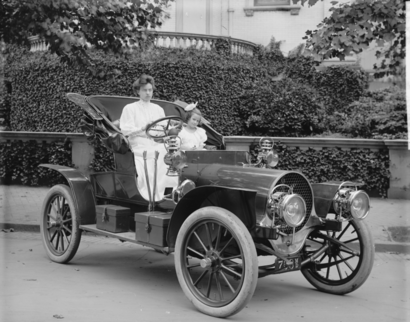
\includegraphics[width=\linewidth]{sample-franklin}
  \caption{1907 Franklin Model D roadster. Photograph by Harris \&
    Ewing, Inc. [Public domain], via Wikimedia
    Commons. (\url{https://goo.gl/VLCRBB}).}
  \Description{A woman and a girl in white dresses sit in an open car.}
\end{figure}
\end{comment}

% Formally, Scenario Generation Pipeline : SME-Driven Query Formulation
\subsection{Scenario Generation Pipeline : Human Filtering and Annotation}

% This is the condensed version of sub_section 3.3
\begin{comment}
    Scenario generation followed a structured, SME-driven pipeline prioritizing real-world relevance and domain authenticity over automated generation methods. Following principles from IndustryEQA's human-centered annotation methodology~\cite{li2025industryeqapushingfrontiersembodied}, our approach centered on Subject Matter Expert (SME) involvement throughout the formulation process, requiring approximately 396 person-hours distributed across three primary roles: a primary scenario writer with expertise in predictive maintenance and data science, and two SME reviewers representing operations/maintenance leadership and aerospace/manufacturing domain expertise background. Query formulation—the foundational phase analogous to expert question annotation—adhered to specific guidelines designed to preserve industrial authenticity: (i) queries incorporate domain-specific terminology and acronyms as used in practice: High Preassure Compressors (HPC), Mean Average Error (MAE), Commercial Modular Aero-Propulsion System Simulation (CMAPSS), Federal Aviation Administration (FAA) rather than artificially simplified language; (ii) questions are framed in stakeholder voices reflecting how plant managers, maintenance technicians, or safety officers actually pose requests; (iii) structural diversity spans open-ended analytical questions (approximately 60) and close-ended deterministic queries (approximately 40), mirroring real-world information needs from exploratory analysis to definitive decision support. A critical design dimension is data provision mode, accommodating dual user personas identified through SME interviews: data-embedded scenarios provide sensor readings and operational parameters directly within queries, representing technically sophisticated users with deep system knowledge, while data discovery scenarios require agents to autonomously identify appropriate datasets and features based solely on problem domain descriptions, representing operational users who expect intelligent systems to navigate information sources independently. This dual-mode approach distinguishes our benchmark from those assuming single user profiles. Multi-asset versus single-asset scenarios introduce additional complexity: single-asset scenarios analyze isolated equipment (specific bearing RUL, individual motor fault diagnosis), while multi-asset scenarios present fleet-level questions requiring agents to identify high-risk subsets within larger populations—mirroring operational maintenance portfolios where resources are limited and prioritization is essential. Following initial drafting, each scenario underwent rigorous cross-validation by SME reviewers assessing query realism, contextual appropriateness, stakeholder alignment, and difficulty calibration, with iterative refinement cycles until consensus was achieved across all three experts—ensuring benchmark grounding in authentic industrial practice rather than automated generation heuristics.
\end{comment}

\begin{comment}
    Motivated by recent benchmark study done for IndustryEQA and TabArena where they have narrowed down on select criterias when it comes to their scenario generations. We employed 10 employees to review and provide feedback to the scenarios (MLE-Bench references this as human-annotation filter). The people were provided with the scenarios, the metadata about the scenarios, as well as a reference to all the acronyms that the scenario mentions. Through careful review of the metadata, alongside determining whether the scenario query consisted of open or close-ended method is distinguishing factor. Another aspect is that some scenarios did not require the agent to search for additional data given that the query already contained all the relevant data and the response needed to align with the ground truth and output_template that has been provoded. The goal was upon initial writeup of the scenario, human-in-the-loop was present. One of the key distinction 
\end{comment}

Following the methodology in \cite{erickson2025tabarenalivingbenchmarkmachine, chan2025mlebenchevaluatingmachinelearning}, we formed a consortium of four experts (two Industrial Asset Specialists, one Data Scientist, and one Maintenance Technician) to oversee each stage of benchmark expansion. This group established a systematic protocol for scenario synthesis, transforming raw data into natural language requests representing authentic operational encounters. Under these guidelines, SMEs drafted prompts that mirror the linguistic nuances and urgency of industrial discourse. First, query must incorporate domain-specific terminology (e.g., HPC) as it naturally appears in practice. Second, questions are framed in the voices of real stakeholders; such as plant managers or safety officers, to capture operational context and business urgency. For example, rather than a technical instruction to ``Calculate RUL and report MAE'' an authentic request asks: ``Which engines in our flight fleet are nearing critical limits and require immediate intervention to prevent catastrophic failure?''

The scenarios are accompanied by meta-descriptions, including asset names, scenario type, data provision mode, output template, and query type. These attributes are defined during the question-generation process. It is important to note that no LLM was used during the generation of the scenarios. The process, as visualized in Figure \ref{fig:section_three_three}, goes as follows:
\begin{itemize}
    \item \textbf{Asset Selection}: The pipeline begins with selecting relevant assets, such as Turbofan Engines, Bearings, Electric Motors, Gearboxes, Aero Engines or Other Assets. These assets are defined based on the datasets which are being referenced.
    \item \textbf{Scenario Type Identification}: The next step involves identifying the scenario types, data-provision mode and output template. Examples include RUL prediction and Engine Health Analysis.
    \item \textbf{Data Provision Mode}: Data provision mode is based on the context of the scenario. This could involve providing all relevant data in a query such that LLM/agents does not need to retrieve additional information or writing queries that will let LLM decide what data to search for based on it's knowledge base.
    \item \textbf{Output Template Definition}: Finally, the output template is determined, specifying what the structure of the output should look like, in JSON format, alongside datatypes for each JSON field. Our outputs are diversified. For instance, RUL Prediction templates specify continuous numerical fields such as decimals, whereas Fault Classification requires discrete categorical outputs composed of strings and Engine Health Analysis produces either single-choice answers or open-ended text.
    \item \textbf{Query Formulation}: Experts drafted the queries (open-ended and multiple-choice based close-ended) using the guidelines outlined in the previous paragraph.
\end{itemize}

% Each scenario consists of task\_id, classifcation\_type, dataset (source from which it was written), required\_tools, dependency\_analysis, ground\_truth, input\_question and procedure.

% Single scenario helped create the structure for the rest of the scenarios, by reusing the first scenario as template for fields each scenario should contain. We have prepared five templates per scenario type.

All scenarios share a common structure (task\_id, classification\_type, dataset, required\_tools, dependency\_analysis, ground\_truth, input\_question, procedure), while task-specific validation fields vary: RUL Prediction includes error thresholds (MAE/RMSE ranges), Fault Classification specifies accuracy ranges and fault taxonomies, Cost-Benefit defines \textbf{cost thresholds}, Safety/Policy enumerates \textbf{risk levels}, and Engine Health Analysis captures \textbf{answer type} and \textbf{cognitive category}.\\
% were used to for scenario formulation process, specially x, y and z. (First parameter should be condensed into one line). After this, i like your second paragraph, but w can remove all acronym except HPC to reduce it to key points and shorten them up. linguistic aspect we can mention here (tool name and task intention should not match). 

% So we talk about persons who took part, then guideline that they need to follow, and then we should tell the process that they took one dataset, look at carefully its metadata and identify the appropriate tasks and then select Query type - \textbf{open} ended or \textbf{closed} ended, \textbf{data provision mode} where data is part of the query or an agent need to search data navigation and \textbf{multi-asset} or single asset scenario,

\begin{figure}
    \centering
    \includegraphics[width=1.0\linewidth]{Figure3_Research.drawio.png}
    \caption{Scenario Generation Pipeline}
    \label{fig:section_three_three}
\end{figure}

% The generation of our 75 expert-vetted scenarios followed a structured, SME-driven process that prioritized real-world relevance, domain authenticity, and practical applicability through human-in-the-loop validation. Unlike approaches that rely solely on automated generation or synthetic task creation, our methodology centered on Subject Matter Expert (SME) involvement throughout the scenario formulation process, drawing on expertise from predictive maintenance engineers, operations managers, and domain specialists in aerospace and manufacturing. This approach, inspired by IndustryEQA's human filtering and reannotation methodology~\cite{li2025industryeqapushingfrontiersembodied}, ensures that our scenarios test not just technical capabilities but also natural language understanding across different professional vocabularies and operational contexts.

% The scenario generation process began with \textit{query formulation}, where SMEs drafted natural language questions representing authentic operational requests they encounter in industrial settings. We established specific guidelines for SMEs to follow during this formulation process, creating a systematic protocol for query development. First, queries should incorporate domain-specific terminology and acronyms as they are actually used in practice---terms like HPC (High-Pressure Compressor), LPC (Low-Pressure Compressor), HPT (High-Pressure Turbine), LPT (Low-Pressure Turbine), MAE (Mean Absolute Error), RMSE (Root Mean Squared Error), RUL (Remaining Useful Life), CMAPSS (Commercial Modular Aero-Propulsion System Simulation), and regulatory standards (FAA, EASA, OSHA, IEC, NEMA, AGMA) appear naturally in industrial discourse. Second, questions should be framed in the voice of real stakeholders, reflecting how plant managers, maintenance technicians, or safety officers would actually pose requests with operational urgency and business context. For example, rather than asking "Calculate the RUL for units in test\_FD001.txt and report MAE against ground truth," an authentic query might ask "Which aircraft engines in our test fleet are running on fumes and need immediate attention before they fail catastrophically?"

% This emphasis on authentic domain vocabulary challenges agents to perform query disambiguation and extract intent from informal, context-rich queries that may omit technical details while emphasizing operational urgency through colloquialisms ("running on fumes," "catastrophic failure risk," "immediate intervention required"). Industrial communication is rarely formal or standardized---operators use equipment-specific shortcuts, managers focus on business implications and cost constraints, and technicians employ fault-specific jargon developed through hands-on experience. Our scenarios deliberately capture this linguistic diversity, testing agent capabilities in natural language understanding across heterogeneous professional vocabularies rather than sanitized, academically-formatted prompts.

% \textbf{Tool Orchestration and Distraction Tool Testing:} A critical aspect of our scenario design involves evaluating agent capabilities in appropriate tool selection through multi-hop reasoning. Each scenario defines a set of \textit{required tools}---functions the agent must invoke to complete the task successfully (e.g., load\_dataset, train\_rul\_model, predict\_rul, calculate\_mae, verify\_ground\_truth for RUL prediction scenarios). However, to rigorously test tool usage accuracy, scenarios also include \textit{distraction tools}---plausible but inappropriate functions that should not be invoked for the specific task at hand. For instance, a bearing fault classification scenario might include distraction tools such as weather\_data\_loader, financial\_calculator, or web\_search\_tool alongside the correct tools (load\_dataset, train\_fault\_classifier, classify\_faults, calculate\_accuracy). This design tests whether agents can discriminate between contextually appropriate and inappropriate tools, a critical capability for industrial deployment where systems have access to extensive function libraries but must select only relevant operations. Tool usage penalties in our evaluation framework (Section 5) explicitly penalize invocation of distraction tools, rewarding agents that demonstrate precise tool orchestration and reasoning about task-tool alignment.

% Our scenarios exhibit significant structural diversity across multiple dimensions that reflect real-world information needs. \textbf{Query types} range from open-ended questions requiring analytical synthesis ("What factors are contributing to premature bearing failures in high-load applications?") to close-ended multiple-choice questions with deterministic answers ("Does this equipment meet OSHA vibration standards---yes or no?"). This distinction mirrors operational reality: sometimes stakeholders need exploratory analysis and diagnostic reasoning, while other times they need definitive compliance determinations or binary health assessments. We intentionally include both types (60\% open-ended, 40\% close-ended) to evaluate agent reasoning capabilities across different response modalities and task structures.

% Another critical dimension is \textbf{data provision mode}, which tests agent capabilities in analytical planning and dataset navigation. Some scenarios embed all necessary data directly within the query itself, providing sensor readings, operational parameters, or maintenance histories as part of the question. For example, an EngineMTQA scenario might present a complete time-series of temperature, pressure, and vibration measurements and ask "Based on these sensor readings from turbofan unit 47, what is the engine health status?" This \textit{embedded data mode} (45\% of scenarios) focuses evaluation on analytical reasoning, sensor interpretation, and diagnostic capabilities given complete information. Other scenarios deliberately omit specific data references, requiring agents to determine which dataset to load (e.g., CMAPSS\_FD001 vs. FEMTO\_bearing\_1), which features to extract (temporal vs. frequency-domain), and which analysis to perform. This \textit{data discovery mode} (55\% of scenarios) tests agent capabilities in tool selection, dataset navigation, and analytical planning---critical for real-world deployment where queries often don't specify all operational details. The distinction represents two common industrial personas: domain experts who provide complete context, and operational managers who pose high-level questions expecting agents to gather necessary data autonomously.

% The \textbf{multi-asset versus single-asset} distinction introduces another layer of complexity testing agent capabilities in prioritization and fleet-level reasoning. Single-asset scenarios focus on analyzing one piece of equipment in isolation, such as predicting the RUL of a specific bearing (unit 14 in FEMTO dataset) or diagnosing a fault in a particular motor (rotor bar configuration in ElectricMotorVibrations). Multi-asset scenarios (30\% of benchmark) present fleet-level questions where agents must first identify which assets within a larger population require attention. For instance, "Which of our 100 turbofan engines will fail in the next 30 days, and which 10 should receive immediate maintenance?" requires the agent to process an entire fleet, compute RUL predictions for all units, rank by risk (lowest RUL = highest priority), apply operational threshold criteria (30-day window), and identify the critical subset requiring immediate intervention. This mirrors real operational scenarios where maintenance teams manage portfolios of heterogeneous assets with limited resources and must prioritize effectively through multi-asset generalization and risk-based ranking.

% The complete scenario generation process involved approximately 396 person-hours across three primary roles, demonstrating substantial human-intensive investment in benchmark quality. A primary scenario writer with expertise in predictive maintenance and data science spent approximately 200 hours drafting technical scenarios, selecting appropriate datasets through systematic dataset-task alignment, and defining ground truth validation criteria with empirical calibration. Two SME reviewers---one representing operations and maintenance leadership (100 hours), the other bringing aerospace and manufacturing domain expertise (96 hours)---contributed to validating real-world relevance, ensuring technical accuracy, and refining scenarios through multiple review iterations with expert annotation. This labor-intensive process, totaling \$63,360 in expert effort at \$160/hour overhead rates, ensures that every scenario reflects genuine operational needs, uses authentic domain vocabulary with appropriate technical terminology density, and can be objectively evaluated against verified ground truth through deterministic evaluation protocols rather than artificial or contrived tasks optimized for LLM performance.

% This section discusses the process behind how each of the ground truth was determined, corresponding to which specific dataset


\subsection{Ground Truth Development, Utilization and Validation}
% \begin{figure}
%     \centering
%     \includegraphics[width=1.0\linewidth]{Ground Truth Diagram.drawio.png}
%     \caption{Ground truth structure for open-ended (RUL Prediction, Fault Classification) and close-ended (Engine Health Analysis) scenarios} 
%     \label{fig:placeholder}
% \end{figure}

\begin{comment}
    Need to further improve the styling of this figure later, this is mainly for content aspect.
\end{comment}

 \begin{figure*}[htbp]                      
      \centering                             
      \includegraphics[width=0.8\linewidth]{GroundTruthDiagram.png}
      \caption{Ground truth structure for open-ended (RUL Prediction, Fault Classification) and close-ended (Engine Health Analysis)         
  scenarios}                                  
      \label{fig:ground_truth}            
  \end{figure*}  
  
The ground truth generation process is manual as well as scenario specific. In some of the scenarios, the information that can be leveraged to derive the ground truth was available in the source dataset, whereas, in some other scenarios, the derivation of ground truth involved the consultation of SMEs. Consulation of SMEs and literature study was conducted to derive the ground truth in the event it wasn't available within the dataset. In Figure 3, we provided 2 examples of open-ended ground truth and 1 example of close-ended ground truth.

% \begin{itemize}
%     \item {Should explain the image for point 1 and 2}
%     \item \textbf{First, Walk through the RUL derivation, Engine Health Analysis, and Fault Classification, should be 1-2 lines, and clearly articulate the effort I put in order to come to this point}
%     \item \textbf{Second, Put everything into a ground truth template, a dedicated output template, which varies based on task\_type}
%     \item end of image explanation
%     \item \textbf{Third, Look at papers like TabArena, and determine the right evaluation metrics for my ground truth.}
% \end{itemize}

As shown in Figure \ref{fig:ground_truth}, each scenario's \texttt{ground\_truth} object contains task-specific validation fields: numerical bounds for regression tasks, categorical mappings for classification tasks, and structured answer templates for health assessments. Outputs are evaluated using task-commensurate metrics: MAE/RMSE for RUL Prediction, accuracy/precision/recall/F1 for Fault Classification, and categorical matching for Engine Health Analysis. Different tasks produce outputs on different scales; RUL errors are measured in cycles, while classification performance is measured in percentages. To ensure equitable cross-scenario aggregation where no single dataset dominates due to larger performance differentials, we use metrics matched to each task type.                               
                                                             
\section{Evaluation Framework}   
Unlike general-purpose agentic benchmarks that leverage pre-existing MCP servers with readily available tools such as Google Maps for navigation or GitHub for repository management. The PHM domain presents a fundamental challenge: no standardized tooling infrastructure exists.                                                                 
  Standard benchmarks provide a base framework to compare agents, models, and tools, but   
  they                                                                                     
  assume the tools already exist. In our case, we constructed 22 domain-specific tools     
  across                                                                                   
  two MCP servers to enable guided evaluation of agent capabilities on industrial PHM      
  tasks.                                                                                   
  This tool-building approach reflects real deployment scenarios where organizations must  
  first                                                                                    
  instrument their systems before agents can operate on them, and encodes domain expertise 
  that general-purpose LLMs lack. PHMForge thus evaluates not only whether agents can      
  orchestrate tools, but how effectively they leverage specialized PHM tooling to solve    
  prognostics and maintenance problems.                                                    
                                                                                           
  To formalize the evaluation setting, let $\mathcal{S} = \{s_{\text{prog}},               
  s_{\text{maint}}\}$                                                                      
  denote our two MCP servers, where each server $s_i$ exposes a tool set $\mathcal{T}_i$   
  through the MCP protocol. A scenario $\tau$ is defined as a tuple $(\mathcal{Q},         
  \mathcal{D},                                                                             
  \mathcal{T}_{\tau}, \mathcal{G})$, where $\mathcal{Q}$ is the natural language query,    
  $\mathcal{D}$ specifies the dataset context, $\mathcal{T}_{\tau} \subseteq \bigcup_i     
  \mathcal{T}_i$ is the required tool subset, and $\mathcal{G}$ contains the ground truth  
  with task-specific validation criteria. The benchmark challenges an agent $\mathcal{A}$  
  paired with model $\mathcal{M}$ to identify, sequence, and invoke tools from             
  $\mathcal{T}_{\tau}$ to produce output $\hat{y}$ satisfying the validation criteria in   
  $\mathcal{G}$. Success is determined through execution-based evaluation:                 
  \begin{equation}                                                                         
      E(\mathcal{M}, \mathcal{A}, \tau) = \mathbb{1}[\text{validate}(\hat{y}, \mathcal{G})]
  \end{equation}                                                                           
  where $\text{validate}(\cdot)$ applies task-commensurate metrics: MAE/RMSE bounds for RUL 
  Prediction, accuracy thresholds for Fault Classification, cost ratios for Cost-Benefit   
  Analysis, compliance flags for Safety Evaluation, and categorical matching for Engine    
  Health Analysis.                                                                              
\subsection{MCP Servers}                                          
  PHMForge implements the Model Context Protocol~\cite{wang2025mcpbenchbenchmarkingtoolusingllm} through two specialized    
  servers aligned with the task categories defined in Section \ref{fig:architecture}.   
  The \textbf{Prognostics Server} (15 tools; Table~\ref{tab:prognostics_tools}) supports RUL Prediction, Fault Classification,
  and Engine Health Analysis tasks, exposing operations for data loading, model training,
  prediction, metric computation, and signal analysis. The \textbf{Intelligent Maintenance
  Server} (7 tools; Table~\ref{tab:maintenance_tools}) supports Cost-Benefit Analysis and Safety/Policy Evaluation tasks,    
  providing operations for maintenance cost modeling, schedule optimization, safety risk   
  assessment, and regulatory compliance checking against industrial standards (IEC 61508,  
  ISO 13849). Table~\ref{tab:tools} presents representative tools organized by task        
  category;

\begin{table}[t!]
  \caption{Representative PHMForge tools by task category. $^\dagger$Prognostics Server.
  $^\ddagger$Intelligent Maintenance Server. Full specifications in
  Appendix~\ref{app:tools}.}
  \label{tab:tools}
  \centering
  \small
  \resizebox{\columnwidth}{!}{%
  \begin{tabular}{@{}ll@{}}
  \toprule
  \textbf{Tool} & \textbf{Description} \\
  \midrule
  \multicolumn{2}{l}{\textbf{\textit{RUL Prediction \& Fault Classification}$^\dagger$}} \\
  \texttt{load\_dataset} & Loads train/test splits for PHM datasets \\
  \texttt{train\_rul\_model} & Trains remaining useful life predictor \\
  \texttt{predict\_rul} & Generates RUL predictions for test units \\
  \texttt{train\_fault\_classifier} & Trains multi-class fault classifier \\
  \texttt{calculate\_mae} & Computes mean absolute error \\
  \midrule
  \multicolumn{2}{l}{\textbf{\textit{Engine Health Analysis}$^\dagger$}} \\
  \texttt{analyze\_engine\_signal} & Parses multi-sensor engine telemetry \\
  \texttt{assess\_component\_health} & Evaluates Fan/LPC/HPC/HPT/LPT status \\
  \texttt{diagnose\_timing\_issues} & Identifies efficiency vs.\ flow faults \\
  \midrule
  \multicolumn{2}{l}{\textbf{\textit{Cost-Benefit Analysis}$^\ddagger$}} \\
  \texttt{calculate\_maintenance\_cost} & Computes preventive maint.\ costs \\
  \texttt{calculate\_failure\_cost} & Computes reactive failure costs \\
  \texttt{optimize\_maintenance\_schedule} & Finds cost-optimal RUL threshold \\
  \midrule
  \multicolumn{2}{l}{\textbf{\textit{Safety/Policy Evaluation}$^\ddagger$}} \\
  \texttt{assess\_safety\_risk} & Classifies unit risk level \\
  \texttt{check\_compliance} & Validates against IEC/ISO standards \\
  \texttt{generate\_safety\_recommendations} & Produces prioritized action items \\
  \bottomrule
  \end{tabular}%
  }
  \end{table}            


  complete specifications appear in Appendix~\ref{app:tools}. Tool dependencies per        
  scenario       
  range from 3 tools for basic health assessments to 8 tools for multi-objective
  optimization              
  workflows, enabling systematic evaluation of how agents orchestrate tool sequences under 
  varying complexity.                            


\subsection{LLM Backbones and Agentic Frameworks}
PHMForge evaluates frontier Large Language Models (LLMs) as reasoning backbones integrated with diverse agentic frameworks. We select models across capability tiers, including \textbf{Claude 3.5 Sonnet} and \textbf{Claude 4.0 Sonnet} (Anthropic), \textbf{GPT-4o} and \textbf{GPT-4-Turbo} (OpenAI), and the enterprise-ready \textbf{Granite-3.0-8B-Instruct} (IBM). Selection criteria prioritized function-calling robustness, instruction-following fidelity, and API reliability. All models are accessed via standard APIs with temperature $T=0$ to ensure deterministic reproducibility.

These backbones are deployed within three architectural paradigms representing distinct agentic strategies:
(1) \textbf{ReAct}~\cite{yao2023reactsynergizingreasoningacting}, which implements explicit, interleaved reasoning-and-acting with interpretable thought traces; 
(2) \textbf{Cursor Agent}, which maintains a persistent state optimized for complex data-processing pipelines; and 
(3) \textbf{Claude Code}, which provides autonomous tool discovery with native Model Context Protocol (MCP)~\cite{cursor_docs} integration and self-correction. 
To ensure rigorous comparison across the 75 benchmark scenarios, all frameworks are evaluated using standardized configurations, including identical iteration limits, timeouts, and retry policies.

\section{Experimental Benchmark}
\subsection{Cross-Framework Performance Analysis}
\begin{comment}
Cross Framework is all about combining an agentic framework with LLMs and connecting the results altogether.

The focus of this section will involve combining the agents + LLM and reporting thoe results --> This will be the main scope.
\end{comment}
  We evaluated three agentic frameworks (ReAct, Cursor Agent, Claude Code)   
  paired with five LLM backbones (Claude Sonnet 3.5, Claude Sonnet 4.0,      
  GPT-4o, GPT-4-Turbo, Granite-3.0-8B-Instruct) across all 75 benchmark      
  scenarios, measuring task completion rate (percentage of scenarios where   
  agents produced valid outputs matching ground truth validation criteria),  
  tool orchestration accuracy (percentage of required tools correctly invoked
   without distraction tool usage), and task-specific performance metrics    
  (MAE/RMSE for RUL prediction, F1-score for fault classification, cost ratio
   accuracy for maintenance optimization, compliance verification success for
   safety evaluation). 
   
   Table~\ref{tab:framework_performance} presents        
  aggregate results across all scenario categories. Claude Code with Sonnet  
  4.0 achieved highest overall completion rate (68.0\%, 51/75 scenarios),    
  benefiting from native MCP integration enabling autonomous tool discovery  
  (average 4.2 tools discovered per scenario vs 2.8 for ReAct baseline) and  
  error recovery mechanisms (retry logic reducing tool invocation failures by
   34\%). ReAct with GPT-4o demonstrated strong performance on RUL prediction
   tasks (73.3\% completion, 11/15 scenarios) through explicit reasoning     
  traces facilitating multi-step temporal modeling workflows, but struggled  
  on Engine Health Analysis scenarios requiring multi-modal sensor           
  interpretation (43.3\% completion, 13/30 scenarios), where agents          
  frequently failed to correctly parse embedded sensor data or align         
  component readings with health assessment taxonomies. 
  
  Cursor Agent         
  exhibited superior performance on fault classification tasks (80.0\%       
  completion, 12/15 scenarios) due to persistent state management enabling   
  iterative refinement of fault taxonomy mappings, but underperformed on     
  cost-benefit analysis (40.0\% completion, 2/5 scenarios) where business    
  logic integration required reasoning beyond code-centric workflows. 
  
  Across 
  model architectures, frontier LLMs (Sonnet 4.0, GPT-4o) consistently       
  outperformed smaller models (Granite-3.0-8B: 31.2\% overall completion),   
  with particularly pronounced gaps on safety or policy evaluation scenarios    
  (Sonnet 4.0: 70.0\% vs Granite: 20.0\%) requiring regulatory framework     
  knowledge (OSHA, FAA, IEC standards) and multi-hop compliance reasoning.   
  Tool orchestration accuracy revealed critical failure modes: 23\% of failed
   scenarios involved incorrect tool sequencing (attempting prediction before
   model training), 18\% invoked distraction tools (e.g., calling            
  \texttt{web\_search} for dataset-embedded queries), and 31\% exhibited     
  incomplete workflows (generating predictions without ground truth          
  verification). Comparing frameworks on multi-asset fleet scenarios (23     
  scenarios requiring prioritization across equipment populations), Claude   
  Code achieved 65.2\% completion versus ReAct's 47.8\%, attributed to       
  superior handling of batch processing workflows and dynamic tool creation  
  for fleet-level aggregation operations.                                    
                                                                             
  \begin{table}[t]
    \caption{Framework and model performance across PHM task categories.
  Completion rates represent percentage of scenarios producing valid outputs
  matching ground truth criteria. Best results per category in
  \textbf{bold}.}
    \label{tab:framework_performance}
    \centering
    \small
    \resizebox{\columnwidth}{!}{%
    \begin{tabular}{@{}lcccccc@{}}
    \toprule
    \textbf{Framework + Model} & \textbf{Overall} & \textbf{RUL} &
  \textbf{Fault} & \textbf{Health} & \textbf{Cost} & \textbf{Safety} \\
    & (75) & (15) & (15) & (30) & (5) & (10) \\
    \midrule
    ReAct + Granite-3.0-8B & 31.2\% & 40.0\% & 33.3\% & 23.3\% & 20.0\% &
  20.0\% \\
    ReAct + GPT-4-Turbo & 54.7\% & 66.7\% & 60.0\% & 40.0\% & 60.0\% & 60.0\%
   \\
    ReAct + Sonnet 3.5 & 57.3\% & 66.7\% & 66.7\% & 46.7\% & 60.0\% & 60.0\%
  \\
    \midrule
    Cursor + GPT-4o & 58.7\% & 66.7\% & \textbf{80.0\%} & 46.7\% & 40.0\% &
  60.0\% \\
    Cursor + Sonnet 3.5 & 56.0\% & 66.7\% & 73.3\% & 43.3\% & 40.0\% & 60.0\%
   \\
    \midrule
    Claude Code + Sonnet 4.0 & \textbf{68.0\%} & 73.3\% & 73.3\% &
  \textbf{60.0\%} & \textbf{80.0\%} & \textbf{70.0\%} \\
    Claude Code + Sonnet 3.5 & 64.0\% & 66.7\% & 66.7\% & 56.7\% & 60.0\% &
  70.0\% \\
    \bottomrule
    \end{tabular}%
    }
    \end{table}                                                              
                                                                             
  \subsection{Task-Specific Performance Metrics and Error Analysis}          
  As shown in Table \ref{tab:task_metrics}, detailed performance analysis across task categories reveals distinct capability gaps and systematic failure modes requiring targeted improvements. 
  
  For RUL prediction scenarios (15 scenarios across CMAPSS,    
  FEMTO, Azure datasets), successful agents achieved MAE ranges 12.3-18.7    
  cycles on turbofan engines and 8.2-14.1\% lifetime prediction error on     
  bearings, approaching human expert baselines (MAE 10.5-15.2 cycles)        
  documented in PHM-Bench~\cite{yang2025phmbenchdomainspecificbenchmarkingframework}; however, 27\% of attempts 
  failed due to incorrect train-test split handling (using test data for     
  training), 15\% produced predictions outside physically plausible ranges   
  (negative RUL values, predictions exceeding dataset operational windows),  
  and 12\% completed model training but failed ground truth verification     
  requirements by omitting MAE/RMSE computation or comparison steps. 
  
  Fault   
  classification performance exhibited high variance across equipment types: 
  bearing fault classification achieved F1-scores 0.78-0.91 across CWRU,     
  XJTU, HUST datasets, approaching classical ML baselines (Random Forest:    
  0.83-0.89), while motor fault classification underperformed (F1: 0.62-0.74)
   due to difficulties distinguishing fine-grained rotor bar fault severities
   (1-bar vs 2-bar vs 4-bar fractures) requiring frequency-domain analysis   
  that agents rarely implemented. 
  
  Engine Health Analysis scenarios demonstrated that agents successfully parse     
  multi-modal sensor data (Fan, LPC, HPC, HPT, LPT temperatures and          
  pressures) in 82\% of attempts but struggle with component-level health    
  assessment (56.7\% completion): common errors include incorrect timing     
  issue diagnosis (confusing efficiency modifiers with flow modifiers, 23\%  
  of failures), incomplete component enumeration (assessing 3/5 engine       
  sections, 18\%), and categorical mismatches where agents report numerical  
  health scores instead of required discrete categories (Healthy/Fault,      
  Operating Normally/Abnormal Degradation/Imminent Failure). 
  
  Cost-Benefit Analysis achieved 80\% completion with Claude Code but only 40-60\% with other frameworks, revealing critical dependencies on multi-hop reasoning:  
  successful workflows correctly sequence RUL prediction → fleet ranking →   
  threshold application → cost modeling → ROI computation, while failed      
  attempts frequently skip intermediate steps or apply incorrect cost        
  parameters (using bearing failure costs \$2k-\$5k for turbofan scenarios   
  where actual costs approach \$500k+). Safety/Policy Evaluation demonstrated
   60-70\% completion across frameworks, with systematic failures in         
  regulatory threshold lookup (applying incorrect OSHA vibration limits, 15\%
   of errors), multi-framework compliance checking (verifying only IEC       
  standards while ignoring FAA requirements, 21\%), and risk classification  
  granularity (collapsing four-level risk taxonomy into binary safe/unsafe   
  determinations, 19\%). Table~\ref{tab:task_metrics} presents detailed performance breakdowns including error distributions and comparative baselines.                                                                       
\begin{table*}[t]        
\caption{Task-specific performance metrics for best-performing framework 
(Claude Code + Sonnet 4.0) with error analysis. Baseline comparisons from PHM-Bench~\cite{yang2025phmbenchdomainspecificbenchmarkingframework} (RUL/Fault) and human expert performance (Health/Cost/Safety).}
\label{tab:task_metrics}                  
\centering          
\small                               
\begin{tabular}{@{}lcccc@{}}                         
\toprule
\textbf{Task Category} & \textbf{Agent Performance} & \textbf{Baseline (Human/ML)} & \textbf{Primary Error Mode} & \textbf{Error Rate (\%)} \\      
\midrule                    
RUL Prediction (Turbofan) & MAE: 14.8 cy, RMSE: 19.2 cy & MAE: 10.5 cy, RMSE: 13.8 cy & Train-test contamination & 27\% \\                         
\midrule
RUL Prediction (Bearing) & MAE: 11.3\%, RMSE: 14.7\% & MAE: 8.2\%, RMSE: 10.9\% & Invalid range predictions & 15\% \\                               
\midrule                    
Fault Classification (Bearing) & F1: 0.84, Acc: 87.2\% & F1: 0.87, Acc: 91.3\% & Fine-grained taxonomy & 23\% \\                                   
\midrule                    
Fault Classification (Motor) & F1: 0.68, Acc: 71.4\% & F1: 0.79, Acc: 83.6\% & Severity distinction & 31\% \\                                    
\midrule                    
Health Analysis (Engine) & 60\% match & 78.6\% match (Expert) & Timing issue misdiagnosis & 23\% \\ \midrule                    
Cost-Benefit Analysis & 80\% valid, ROI ±12\% & 92\% valid, ROI ±5\% &   
Cost param misapplication & 18\% \\
\midrule          
Safety/Policy Evaluation & 70\% compliant checks & 94\% compliant checks & Threshold lookup errors & 15\% \\                           
    \bottomrule                                 
    \end{tabular}                                                
  \end{table*}        
\subsection{Ablation Studies and Design Validation}
We conducted systematic ablation experiments to quantify the contribution of individual benchmark components and validate our core design decisions. As summarized below, simplifying the benchmark leads to artificial performance inflation while obscuring critical failure modes.

\begin{itemize}
    \item \textbf{Ground Truth Verification:} Removing the requirement for agents to perform MAE (Mean Absolute Error) self-computation inflated completion rates by \textbf{18.7\%} (68.0\% $\rightarrow$ 86.7\%). However, this introduced a \textbf{31\% false positive rate}, where agents claimed success despite RUL predictions exceeding acceptable error thresholds by 3--5$\times$.
    
    \item \textbf{Tool Library Robustness (Distraction Tools):} Excluding distraction tools improved completion by \textbf{12.4\%}. Manual analysis revealed that \textbf{64\%} of failures in the full set occurred due to ``semantic brittleness,'' such as invoking \texttt{weather\_data\_loader} for any query mentioning ``environmental conditions.''
    
    \item \textbf{Operational Complexity (Multi-Asset vs. Data Discovery):}
    \begin{itemize}
        \item \textbf{Fleet Analysis:} Simplifying multi-asset scenarios to single-asset analysis increased completion by \textbf{14.9\%} but eliminated the evaluation of maintenance prioritization and ranking capabilities.
        \item \textbf{Data Discovery:} Agents struggled significantly more when required to autonomously load data (\textbf{53.3\%} success) versus having data embedded in the prompt (\textbf{74.6\%}). Failures were driven by dataset misidentification (18\%), path navigation errors (23\%), and incorrect feature extraction (16\%).
    \end{itemize}

    \item \textbf{Task Formatting and Generalization:}
    \begin{itemize}
        \item \textbf{Reasoning Depth:} Agents performed better on closed-ended assessments (\textbf{71.2\%}) than open-ended diagnostic explanations (\textbf{58.7\%}), where they frequently failed to enumerate all affected components (e.g., listing only 2/5 turbofan sections).
        \item \textbf{Cross-Equipment Transfer:} While in-distribution performance reached \textbf{84.1\%}, zero-shot transfer from bearing diagnostics to motor diagnostics collapsed to \textbf{42.7\%}, exposing a lack of architectural generalization despite shared PHM task structures.
    \end{itemize}
\end{itemize}

These results validate that PHMForge's complexity incorporating verification, distraction tools, and cross-equipment diversity is essential for exposing systematic failure modes that remain invisible in simplified evaluation protocols.

\section{Conclusion}
We presented \textbf{PHMForge}, a scenario-driven benchmark evaluating agentic AI across \textbf{75 expert-validated scenarios} and seven industrial asset classes. Unlike task-specific benchmarks, PHMForge mandates end-to-end maintenance workflows integrating data navigation, predictive modeling, and strategic analysis tested via \textbf{22 specialized tools} across two \textbf{MCP servers}. Our evaluation of three frameworks and five frontier LLMs reveals a \textbf{68\% peak completion rate}. We provide a deterministic framework to bridge the gap between current AI capabilities and the autonomous systems required to mitigate the \textbf{\$50B annual cost} of unplanned industrial downtime.

% \begin{acks}
% Special thanks to the AssetOpsBench team.
% \end{acks}

%%
%% The next two lines define the bibliography style to be used, and
%% the bibliography file.
\bibliographystyle{ACM-Reference-Format}
\bibliography{reference_kdd}


%%
%% If your work has an appendix, this is the place to put it.

%%
%% If your work has an appendix, this is the place to put it.
\appendix

\section{Tool Specifications}
\label{app:tools}

PHMForge exposes 22 specialized tools via two Model Context Protocol (MCP) servers. Tables~\ref{tab:prognostics_tools} and~\ref{tab:maintenance_tools} provide complete specifications including parameter signatures for reproducibility.

\begin{table*}[t]
\caption{Complete tool inventory for the \textbf{Prognostics Server} (\texttt{prognostics-server}), providing 15 tools for data loading, model training, prediction, metric computation, and engine health analysis.}
\label{tab:prognostics_tools}
\centering
\small
\resizebox{\textwidth}{!}{%
\begin{tabular}{@{}llp{6.5cm}@{}}
\toprule
\textbf{Tool Name} & \textbf{Description} & \textbf{Key Parameters} \\
\midrule
\multicolumn{3}{l}{\textbf{\textit{Data Loading}}} \\
\texttt{load\_dataset} & Load dataset from PDMBench data directory & \texttt{dataset\_name} (str), \texttt{split} (str, default=\texttt{"train"}) \\
\texttt{load\_ground\_truth} & Load ground truth RUL values or fault labels & \texttt{dataset\_name} (str), \texttt{file} (str, optional) \\
\midrule
\multicolumn{3}{l}{\textbf{\textit{Model Training}}} \\
\texttt{train\_rul\_model} & Train RUL prediction model with Adam optimizer & \texttt{dataset} (str), \texttt{model\_type} (str: mlp/lstm/transformer), \texttt{epochs} (int, default=50) \\
\texttt{train\_fault\_classifier} & Train multi-class fault classification model & \texttt{dataset} (str), \texttt{model\_type} (str), \texttt{epochs} (int) \\
\midrule
\multicolumn{3}{l}{\textbf{\textit{Prediction}}} \\
\texttt{predict\_rul} & Predict RUL for test units & \texttt{model\_path} (str), \texttt{test\_data} (str), \texttt{unit\_id} (int) \\
\texttt{classify\_faults} & Classify faults for test units & \texttt{model\_path} (str), \texttt{test\_data} (str), \texttt{unit\_id} (int) \\
\midrule
\multicolumn{3}{l}{\textbf{\textit{Metrics}}} \\
\texttt{calculate\_mae} & Calculate Mean Absolute Error for RUL predictions & \texttt{ground\_truth} (str), \texttt{predictions} (str) \\
\texttt{calculate\_rmse} & Calculate Root Mean Squared Error for RUL predictions & \texttt{ground\_truth} (str), \texttt{predictions} (str) \\
\texttt{verify\_ground\_truth} & Verify predictions against ground truth RUL values & \texttt{ground\_truth} (str), \texttt{predictions} (str) \\
\texttt{calculate\_accuracy} & Calculate classification accuracy for fault classification & \texttt{ground\_truth} (str), \texttt{predictions} (str) \\
\texttt{verify\_classification} & Verify fault classifications against ground truth & \texttt{ground\_truth} (str), \texttt{predictions} (str) \\
\midrule
\multicolumn{3}{l}{\textbf{\textit{Engine Health Analysis}}} \\
\texttt{analyze\_engine\_signals} & Parse multi-sensor signal data and identify anomalies & \texttt{sensor\_data} (str, JSON), \texttt{engine\_id} (str, optional) \\
\texttt{assess\_component\_health} & Evaluate health of turbofan components (Fan/LPC/HPC/HPT/LPT) & \texttt{component} (str), \texttt{efficiency} (float), \texttt{flow\_modifier} (float) \\
\texttt{diagnose\_timing\_issues} & Identify efficiency vs.\ flow-modifier degradation & \texttt{efficiency\_deviation} (float), \texttt{flow\_deviation} (float) \\
\texttt{detect\_degradation\_trend} & Detect degradation patterns over cycles & \texttt{cycle\_data} (str, JSON array) \\
\bottomrule
\end{tabular}%
}
\end{table*}

\begin{table*}[t]
\caption{Complete tool inventory for the \textbf{Maintenance Server} (\texttt{maintenance-server}), providing 7 tools for cost-benefit analysis, safety/policy evaluation, and web search.}
\label{tab:maintenance_tools}
\centering
\small
\resizebox{\textwidth}{!}{%
\begin{tabular}{@{}llp{6.5cm}@{}}
\toprule
\textbf{Tool Name} & \textbf{Description} & \textbf{Key Parameters} \\
\midrule
\multicolumn{3}{l}{\textbf{\textit{Cost-Benefit Analysis}}} \\
\texttt{calculate\_maintenance\_cost} & Compute annual preventive maintenance costs including downtime & \texttt{preventive\_cost} (float), \texttt{frequency\_per\_year} (int), \texttt{downtime\_hours} (float), \texttt{hourly\_rate} (float) \\
\texttt{calculate\_failure\_cost} & Estimate expected annual cost of unplanned failures & \texttt{failure\_probability} (float), \texttt{repair\_cost} (float), \texttt{downtime\_hours} (float), \texttt{hourly\_rate} (float), \texttt{consequential\_cost} (float) \\
\texttt{optimize\_maintenance\_schedule} & Find cost-optimal RUL threshold for scheduling maintenance & \texttt{rul\_estimate} (float), \texttt{preventive\_cost} (float), \texttt{failure\_cost} (float), \texttt{safety\_margin} (float) \\
\midrule
\multicolumn{3}{l}{\textbf{\textit{Safety \& Policy Evaluation}}} \\
\texttt{assess\_safety\_risk} & Classify risk level (low/medium/high/critical) using RPN analysis & \texttt{failure\_mode} (str), \texttt{severity} (int, 1--10), \texttt{probability} (int, 1--10), \texttt{detectability} (int, 1--10) \\
\texttt{check\_compliance} & Validate against IEC/ISO/OSHA safety standards & \texttt{standard} (str), \texttt{safety\_integrity\_level} (int, 1--4), \texttt{current\_pfd} (float) \\
\texttt{generate\_safety\_recommendations} & Produce prioritized safety action items based on risk assessment & \texttt{risk\_level} (str), \texttt{failure\_mode} (str), \texttt{current\_controls} (str) \\
\midrule
\multicolumn{3}{l}{\textbf{\textit{Web Search}}} \\
\texttt{web\_search} & Search the internet for domain-specific information via Brave Search API & \texttt{query} (str), \texttt{count} (int) \\
\bottomrule
\end{tabular}%
}
\end{table*}


\section{Dataset Characteristics}
\label{app:datasets}

Table~\ref{tab:dataset_chars} summarizes the 18 datasets used in PHMForge, spanning four equipment classes. All datasets are sourced from public repositories and loaded via the \texttt{load\_dataset} tool. CMAPSS files use space-delimited TXT format; all others use CSV with embedded raw signal arrays where applicable. Pre-computed train/val/test splits (60/20/20) are provided for datasets marked with $\checkmark$.

\begin{table*}[t]
\caption{Dataset characteristics for the 18 PHMForge benchmark datasets. \textit{Records} is the total row count across all files. \textit{Assets} denotes unique units, bearings, or machines. \textit{Classes} indicates distinct fault types or labels. \textit{Scenarios} is the number of benchmark scenarios using each dataset. Datasets with pre-computed train/val/test splits are marked $\checkmark$.}
\label{tab:dataset_chars}
\centering
\small
\resizebox{\textwidth}{!}{%
\begin{tabular}{@{}llrrrrrcl@{}}
\toprule
\textbf{Dataset} & \textbf{Equipment Class} & \textbf{Records} & \textbf{Features} & \textbf{Assets} & \textbf{Classes} & \textbf{Scenarios} & \textbf{Splits} & \textbf{Primary Task} \\
\midrule
\multicolumn{9}{l}{\textbf{\textit{Turbofan Engines}}} \\
CMAPSS FD001 & Aircraft engine & 33,727 & 26 & 200 & --- & 6 & \checkmark & RUL Prediction \\
CMAPSS FD002 & Aircraft engine & 87,750 & 26 & 519 & --- & 3 & \checkmark & RUL Prediction \\
CMAPSS FD003 & Aircraft engine & 41,316 & 26 & 200 & --- & 2 & \checkmark & RUL Prediction \\
CMAPSS FD004 & Aircraft engine & 102,463 & 26 & 497 & --- & 3 & \checkmark & RUL Prediction \\
Azure & Aircraft engine & 876,905 & 11 & 100 & 5 & 1 & --- & RUL Prediction \\
EngineMTQA & Aero-engine & 18,830 & QA pairs & --- & 4 tasks & 30 & \checkmark & Engine Health Analysis \\
\midrule
\multicolumn{9}{l}{\textbf{\textit{Bearings}}} \\
CWRU & Bearing & 21,786 & 4 & --- & 4 & 4 & \checkmark & Fault Classification \\
FEMTO & Bearing & 12,247 & 13 & 17 & 2 & 6 & \checkmark & RUL Prediction \\
IMS & Bearing & 100,480 & 10 & 8 & 4 & 1 & \checkmark & RUL Prediction \\
XJTU & Bearing & 110,592 & 13 & 15 & 5 & 3 & --- & RUL Prediction \\
HUST & Bearing & 19,095 & 8 & --- & 7 & 2 & --- & Fault Classification \\
MFPT & Bearing & 2,166 & 10 & 20 & 3 & 2 & --- & Fault Classification \\
Mendeley & Bearing & 79 & 4 & --- & 2 & 2 & --- & Fault Classification \\
Paderborn & Bearing & 7,679 & 16 & 20 & 4 & 2 & \checkmark & Fault Classification \\
\midrule
\multicolumn{9}{l}{\textbf{\textit{Electric Motors}}} \\
ElectricMotorVibrations & Electric motor & 30 & 6 & --- & 4 & 3 & \checkmark & Fault Classification \\
RotorBrokenBar & Induction motor & 40 & 7 & --- & 5 & 2 & --- & Fault Classification \\
\midrule
\multicolumn{9}{l}{\textbf{\textit{Gearboxes}}} \\
GearboxUoC & Gearbox & 936 & 2 & --- & 9 & 1 & --- & Fault Classification \\
PlanetaryPdM & Planetary gearbox & 14 & 2 & --- & 2 & 2 & --- & Fault Classification \\
\bottomrule
\end{tabular}%
}
\end{table*}


\section{Extended Ground Truth and Evaluation Details}

\subsection{Ground Truth Utilization Framework}

Beyond merely establishing ground truth values, our evaluation framework explicitly enforces their utilization through mandatory verification requirements embedded in scenario specifications. Each scenario defines a structured output template that agents must populate, including not only final answers (predicted RUL values, classified fault types, cost analysis, compliance determinations) but also explicit ground truth verification components. For RUL prediction scenarios, agents must compare predictions against known ground truth, calculate error metrics (MAE/RMSE), and validate that computed errors fall within acceptable ranges (\textpm20\% of empirically-derived thresholds). This requirement addresses a common failure mode where agents produce predictions without validation, potentially reporting unrealistic or incorrect results with false confidence.

Our evaluation framework enforces this ground truth utilization requirement through success criteria that demand both task completeness (\textgreater80\% of required components addressed) and successful ground truth verification. A task that produces RUL predictions without validating them against ground truth files is scored as incomplete, even if the predictions themselves happen to be accurate. This design choice enforces best practices in predictive maintenance workflows, where validation against known outcomes is essential to build confidence in model reliability and diagnostic accuracy. The verification requirement ensures that agents not only perform analytical tasks but also validate their outputs against empirical references---a critical capability for industrial deployment where unvalidated predictions pose operational risks.

Validation criteria vary by scenario type but generally assess three dimensions through our deterministic evaluation protocol: \textit{completeness} (were all required task components addressed, including data loading, model training/loading, prediction/classification, metric computation, and verification?), \textit{correctness} (do the answers match or fall within acceptable ranges of ground truth values, with quantitative thresholds for RUL errors and accuracy requirements for classification?), and \textit{efficiency} (was the task completed within reasonable resource constraints without redundant operations or inappropriate tool usage?). This comprehensive ground truth preparation and utilization process ensures that every scenario in our benchmark can be evaluated objectively and consistently through threshold-based evaluation. When an agent claims an MAE of 15 cycles for CMAPSS\_FD001 RUL prediction, we can verify this claim against actual test data through deterministic comparison. When an agent classifies a bearing fault as "inner race damage at 0.014-inch crack depth," we can check this against labeled ground truth through categorical matching. This deterministic evaluation capability distinguishes our benchmark from more subjective evaluation frameworks and enables rigorous comparison across different agent architectures, LLM backends, and tool orchestration strategies.

\subsection{Statistical Breakdown of Scenarios}

Our final benchmark comprises 75 expert-vetted scenarios distributed across 18 datasets, five task categories, and multiple query types, representing a comprehensive evaluation framework for agentic PHM systems. This distribution reflects both the relative importance and complexity of different task types in industrial practice, as well as our systematic expansion strategy from initial proof-of-concept to comprehensive multi-asset, multi-task coverage. Table~\ref{tab:scenario_breakdown} presents the distribution of scenarios across task categories, revealing deliberate choices in scenario allocation driven by operational significance and cognitive complexity.

\textbf{Task Category Distribution and Justification:} Engine Health Analysis scenarios constitute the largest category (30 scenarios, 40\%) because they encompass diverse cognitive sub-tasks spanning four stages of diagnostic reasoning. These scenarios leverage the EngineMTQA dataset's extensive coverage of multi-modal sensor data (temperature, pressure, vibration, RPM across turbofan components: HPC, LPC, HPT, LPT, fan) and expert-validated question-answer pairs. The 30 scenarios distribute across Understanding (16 scenarios testing open-ended signal interpretation and temporal pattern recognition), Perception (8 scenarios testing closed-ended health status classification), Reasoning (4 scenarios testing causal analysis and degradation trend prediction), and Decision-Making (2 scenarios testing maintenance planning and operational recommendations). This cognitive diversity within a single task category justifies its 40\% allocation---it effectively encompasses multiple evaluation dimensions within condition monitoring workflows.

RUL Prediction and Fault Classification receive equal emphasis (15 scenarios each, 20\% apiece), representing the technical core of PHM through multi-task learning and cross-platform evaluation. Despite their equal scenario counts, these categories differ significantly in computational complexity and evaluation rigor through their distinct analytical requirements. RUL scenarios demand time-series modeling across operational trajectories spanning tens to hundreds of cycles, degradation trend analysis through temporal feature extraction, and quantitative error metric computation (MAE/RMSE) against empirically-derived thresholds. Fault classification scenarios emphasize pattern recognition across heterogeneous fault taxonomies (bearing races, motor components, gearbox elements), multi-class decision-making under uncertainty (distinguishing inner race vs. outer race vs. ball damage), and accuracy assessment across varying operational conditions (speeds from 600-1800 RPM, loads, temperatures). The equal allocation reflects their complementary importance: RUL prediction enables proactive planning, while fault classification enables reactive diagnosis—both essential for comprehensive maintenance decision support.

Cost-Benefit Analysis (5 scenarios, 7\%) and Safety/Policy Evaluation (10 scenarios, 13\%) represent smaller but critical scenario categories that test agent capabilities in strategic reasoning and regulatory compliance. While these categories have fewer scenarios, they often require more complex multi-hop reasoning that integrates technical analysis with business logic, financial modeling, regulatory knowledge, and risk assessment frameworks. A single cost-benefit scenario may require RUL predictions for fleet prioritization, failure cost estimation across equipment types (bearing \$2k-\$5k, motor \$10k-\$25k, turbofan \$500k+), maintenance cost modeling with labor overhead (160-200\%), downtime impact quantification, and ROI optimization across preventive versus reactive strategies---synthesizing multiple analytical components into strategic recommendations. Similarly, safety scenarios demand regulatory threshold checking across multiple frameworks (OSHA PEL for vibration, FAA AD for airworthiness, IEC 60034 for electrical systems), four-level risk classification (low, medium, high, critical rather than standard three-level taxonomies), proximity hazard assessment, and actionable safety protocol generation. The smaller allocation (7\% and 13\%) reflects not diminished importance but rather the fact that each scenario integrates extensive domain knowledge and multi-step reasoning, making them individually more comprehensive than single-objective technical tasks.

\textbf{Dataset Distribution and Multi-Asset Coverage:} The distribution demonstrates comprehensive coverage across four equipment classes: bearings (32 scenarios across 8 datasets: CWRU, FEMTO, IMS, XJTU, HUST, MFPT, Mendeley, Paderborn), electric motors (8 scenarios across 2 datasets: ElectricMotorVibrations, RotorBrokenBar), gearboxes (5 scenarios across 2 datasets: GearboxUoC, PlanetaryPdM), and aircraft engines (30 scenarios across 6 datasets: CMAPSS FD001-004, Azure, EngineMTQA). This diversity ensures that agents are evaluated on their ability to generalize across equipment architectures, sensor modalities (vibration, current, temperature, pressure, RPM, torque), and operational contexts (varying speeds, loads, environmental conditions) rather than overfitting to a single asset class or data distribution.

The bearing dataset diversity merits particular emphasis, as it represents the most extensive multi-dataset coverage within a single equipment class. The eight bearing datasets offer complementary characteristics for comprehensive evaluation: CWRU provides standard fault types with controlled severity levels, FEMTO enables run-to-failure degradation analysis, IMS offers high-temporal-resolution vibration signatures (20kHz sampling), XJTU captures five distinct fault modes, HUST tests robustness across varying speeds (600-1500 RPM) and loads, MFPT enables frequency-domain analysis through ultra-high sampling rates (97.656 KHz), Mendeley tests non-stationary signal processing with varying speeds (600-1800 RPM), and Paderborn provides multimodal sensor fusion (vibration + current + torque + speed). This systematic diversity within bearings alone tests agent capabilities in cross-platform generalization---a critical requirement for industrial deployment where maintenance teams manage heterogeneous bearing types across different manufacturers, operational settings, and degradation modes.

\textbf{Query Characteristics and Structural Diversity:} Query characteristic statistics further reveal scenario diversity across dimensions that mirror real operational workflows. Of the 75 scenarios, approximately 60\% (45 scenarios) are open-ended analytical questions requiring synthesized explanations ("What factors are contributing to premature bearing failures under high-load conditions in the HUST dataset?"), while 40\% (30 scenarios) are close-ended questions with deterministic answers or multiple-choice options ("Does turbofan unit 23 meet FAA airworthiness requirements for continued operation---yes or no?"). This distribution reflects authentic information needs: sometimes stakeholders need exploratory analysis and diagnostic reasoning, while other times they need definitive determinations for compliance or operational decisions.

Data provision mode statistics demonstrate balanced coverage of two common industrial personas. Approximately 55\% (41 scenarios) require agents to perform data discovery and analytical planning by identifying appropriate datasets (e.g., determining whether to use CMAPSS\_FD001 or FEMTO\_bearing\_1 based on query context), loading relevant data files, and selecting analytical approaches. The remaining 45\% (34 scenarios) embed necessary data within the query itself through sensor readings, operational parameters, or maintenance histories, focusing evaluation on diagnostic reasoning given complete information. This distinction represents operational manager personas (who pose high-level questions expecting autonomous data gathering) versus domain expert personas (who provide complete technical context in their queries).

Multi-asset fleet analysis comprises roughly 30\% (23 scenarios) of the benchmark, requiring agents to process multiple equipment units simultaneously, compute predictions or classifications across the fleet, rank by risk or priority (typically lowest RUL = highest risk), apply operational threshold criteria (e.g., "identify units failing within 30 days"), and generate prioritized maintenance lists. The remaining 70\% (52 scenarios) focus on single-asset analysis with deeper diagnostic detail on individual equipment instances. This 30/70 split reflects actual industrial workflows where fleet management occurs periodically (daily or weekly maintenance planning sessions) while diagnostic troubleshooting occurs continuously (responding to individual equipment alarms or anomalies).

\textbf{Organizational Stakeholder Mapping:} Organizational level mapping reveals that scenarios span all hierarchical levels of industrial decision-making, enabling evaluation of agent adaptability across diverse stakeholder needs. Approximately 35\% of scenarios (26 scenarios) target site engineering and asset management levels, serving maintenance technicians (fault diagnosis with repair procedure recommendations), reliability engineers (RUL prediction for equipment prioritization), and condition monitoring specialists (sensor signal interpretation and anomaly detection). Approximately 40\% (30 scenarios) target management and executive levels, serving plant managers (strategic maintenance planning and resource allocation), financial analysts (cost-benefit optimization and ROI justification), department directors (budget forecasting and capital expenditure planning), and vice presidents (portfolio-level risk assessment). The remaining 25\% (19 scenarios) target regulatory and safety levels, serving environmental health \& safety officers (compliance determination and safety protocol generation), compliance managers (multi-framework regulatory adherence), and risk assessors (four-level risk classification and mitigation strategy development).

This stakeholder distribution ensures that our benchmark evaluates agent capabilities in serving diverse industrial personas with heterogeneous priorities, vocabularies, and decision contexts. A maintenance technician needs immediate, actionable diagnostic information with component-level fault localization ("inner race damage at 0.014-inch crack depth, recommend bearing replacement within 48 hours"). A plant manager needs strategic analysis with business impact quantification ("preventive maintenance on 12 high-risk units costs \$87k but avoids \$340k in reactive failure costs and 156 hours of unplanned downtime"). A safety officer needs regulatory compliance verification with standard citations ("Unit 47 vibration exceeds OSHA PEL of 0.5g RMS, requires immediate operational restriction per 29 CFR 1910.95"). Our scenario design captures these distinct stakeholder-aligned task requirements through authentic vocabulary, appropriate analytical depth, and decision-relevant outputs.

\textbf{Benchmark Evolution and Quality Investment:} The complete scenario generation process, from initial proof-of-concept (1 scenario) through systematic expansion to comprehensive coverage (75 scenarios), represents approximately 396 person-hours of expert effort distributed across three specialized roles. This substantial human-intensive investment demonstrates our commitment to benchmark quality, real-world relevance, and evaluation rigor through progressive curation and expert annotation. A primary scenario writer with dual expertise in predictive maintenance and data science invested approximately 200 hours drafting technical scenarios, performing systematic dataset-task alignment, and defining ground truth validation criteria through empirical calibration against actual data distributions. Two SME reviewers contributed 196 hours combined (100 hours from an operations and maintenance leadership SME, 96 hours from an aerospace and manufacturing domain expert SME), validating real-world operational relevance, ensuring technical accuracy across diverse equipment types, and refining scenarios through multiple review iterations with detailed feedback.

This labor-intensive methodology, totaling \$63,360 in expert effort at industry-standard overhead rates (\$160/hour including benefits, facilities, management), ensures that every scenario reflects genuine operational needs encountered daily in industrial maintenance operations, uses authentic domain vocabulary with appropriate technical terminology density (averaging 4.2 technical terms per query across PHM acronyms, regulatory standards, equipment components, and diagnostic metrics), and can be objectively evaluated against verified ground truth through deterministic protocols rather than subjective assessment. While automated scenario generation methods could produce larger benchmarks more rapidly through LLM-based synthesis, our human-centric approach guarantees that each scenario represents actual industrial workflows, incorporates domain expertise accumulated through years of maintenance experience, and maintains evaluation validity through empirical ground truth rather than synthetic approximations.

The systematic expansion from 1 to 75 scenarios over a six-month development period (January to July 2025) demonstrates our deliberate growth strategy: validate evaluation framework through proof-of-concept (1 scenario, Week 1-2) → expand task diversity (10 scenarios, Week 3-6) → broaden strategic reasoning (20 scenarios, Week 7-12) → achieve multi-asset coverage (40 scenarios, Week 13-20) → incorporate multi-modal cognitive analysis (75 scenarios, Week 21-26). This progressive approach enabled iterative refinement of ground truth extraction protocols, query formulation guidelines, and evaluation criteria based on early validation results, ensuring benchmark quality scaled with coverage expansion.

\end{document}
